%%-*-latex-*-

\documentclass[wide]{slides}

% Language
%
\usepackage{hyphenat}          % \hyp{} is a breakable dash
\usepackage{alltt}             % Verbatim with macros
\usepackage{booktabs}

\frenchspacing  % Follow French conventions after a period

% Maths
%
\usepackage{stmaryrd}

% Graphics
%
\usepackage{graphicx}

% New environments and commands
%
../TeX/commands.tex
%%-*-latex-*-

\newcommand{\evalf}[2]{\llbracket{#1}\rrbracket{#2}}

% OCaml pieces of source code
%
\newcommand{\phrase}[1]{\texttt{#1}}
\newcommand{\excerpt}[1]{\texttt{#1}}

% O'Caml language
%
\newcommand{\ipat}[1]{\overline{#1}}
\newcommand{\topclos}{\langle{fun}\rangle}

\newcommand{\wild}{{\LARGE \_}}
\newcommand{\kwd}[1]{\textsf{\textbf{#1}}}
\newcommand{\ident}[1]{\textsf{#1}}
\newcommand{\cst}[1]{\textsf{#1}}
\newcommand{\type}[1]{\textsl{#1}}
\newcommand{\str}[1]{\textsf{"#1"}}
\newcommand{\num}[1]{\textsf{#1}}
%\newcommand{\comment}[1]{\textsf{(* #1 *)}}
\newcommand{\camlcons}{\textsf{::}}

\newcommand{\lpar}{\textsf{(}}
\newcommand{\rpar}{\textsf{)}}
\newcommand{\lbra}{\textsf{[}}
\newcommand{\rbra}{\textsf{]}}
\newcommand{\equal}{\textsf{=}\xspace}
\newcommand{\nequal}{\textsf{\footnotesize <>}\xspace}
\newcommand{\assign}{\textsf{:=}\xspace}
\newcommand{\unit}{\textsf{()}\xspace}
\newcommand{\vbar}{\texttt{|}\xspace}

\newcommand{\Xopen}{\kwd{open}\xspace}
\newcommand{\Xlet}{\kwd{let}\xspace}
\newcommand{\Xrec}{\kwd{rec}\xspace}
\newcommand{\Xin}{\kwd{in}\xspace}
\newcommand{\Xfun}{\kwd{fun}\xspace}
\newcommand{\Xfunction}{\kwd{function}\xspace}
\newcommand{\Xmatch}{\kwd{match}\xspace}
\newcommand{\Xtry}{\kwd{try}\xspace}
\newcommand{\Xwith}{\kwd{with}\xspace}
\newcommand{\Xif}{\kwd{if}\xspace}
\newcommand{\Xthen}{\kwd{then}\xspace}
\newcommand{\Xelse}{\kwd{else}\xspace}
\newcommand{\Xtype}{\kwd{type}\xspace}
\newcommand{\Xand}{\kwd{and}\xspace}
\newcommand{\Xof}{\kwd{of}\xspace}
\newcommand{\Xfor}{\kwd{for}\xspace}
\newcommand{\Xwhile}{\kwd{while}\xspace}
\newcommand{\Xdo}{\kwd{do}\xspace}
\newcommand{\Xdone}{\kwd{done}\xspace}
\newcommand{\Xbegin}{\kwd{begin}\xspace}
\newcommand{\Xend}{\kwd{end}\xspace}
\newcommand{\Xexception}{\kwd{exception}\xspace}
\newcommand{\Xas}{\kwd{as}\xspace}
\newcommand{\Xtrue}{\kwd{true}\xspace}
\newcommand{\Xfalse}{\kwd{false}\xspace}

../TeX/ocaml_macros.tex

% ----------------------------------------------------------------
% Document
%
\maintitle{Programming with OCaml}
\mainauthor{\textbf{Christian Rinderknecht}\\
  {\small\url{Christian.Rinderknecht@nomadic-labs.com}}\\
\Nomadic}
\confname{Tezos Masterclass}
\confshortname{Tezos}
\confdate{20 October 2018}

\begin{document}

\maketitle

\begin{slide}
  \title{Introduction}

  \begin{itemize}

    \item Rewrite systems are a good mathematical and mental model for
      understanding functional languages.

    \item It is time now to learn an actual functional language, so we
      can run programs.

    \item The aim of these lectures is to introduce the functional
      language \OCaml, which is used for the core development at
      \Tezos (network protocols, compilers and virtual machines for
      smart contracts).

    %% \item We will build in \OCaml an interpreter for a tiny subset of
    %%   \OCaml itself (\textbf{bootstrapping}).

    %% \item If you like that sort of thing, you would certainly enjoy
    %%   contributing to the core of the \Tezos blockchain.

    \item We are going to start with a mini language that is actually
      a subset of \OCaml, then grow it step by step.

  \end{itemize}

\end{slide}

\begin{slide}
  \title{Growing a language}

  \begin{itemize}

    \item The presentation is principled, that is, it relies on a
      systematic classification of the \textbf{syntactic constructs}
      and their \textbf{formal semantics}.

    \item When we reach a certain complexity, we will drop the formal
      descriptions.

    \item Both theoretical and pragmatic, our approach is
      complementary to those usually found in books.

    %% \item We will demonstrate how good \OCaml is for compiler
    %%   construction by writing an interpreter for our mini language.

    \item Let mini-ML be the name of the subset of \OCaml we are going
      to grow.

  \end{itemize}
\end{slide}

\begin{slide}
  \title{Appending a stack}

  \begin{itemize}

    \item The notation we introduced for stacks in the context of
      rewrite systems actually follows the \OCaml convention.

    \item In the context of functional programming, stacks are often
      called \textbf{lists}.

    \item Here are different ways to express the same list in \OCaml:
      \begin{equation*}
        1::(2::3::(4::\el)) \;\; = \;\; 1::2::3::4::\el \;\; = \;\; [1;2;3;4].
      \end{equation*}

    \item Before starting, let us see how a familiar function defined
      with a rewrite system looks like in \OCaml.

    \item Let us recall the appending of a stack:
      \begin{align*}
        \fun{cat}(        \el,t) &\xrightarrow{\alpha} t\\
        \fun{cat}(\cons{x}{s},t) &\xrightarrow{\smash\beta}
        \cons{x}{\fun{cat}(s,t)}
      \end{align*}

  \end{itemize}
\end{slide}

\begin{slide}
  \title{Appending a stack (continued)}

  \begin{itemize}

    \item In \OCaml, the function name is not repeated (once for each
      rule).

    \item Instead, it is introduced once by a \textbf{binder} called
      \textbf{\texttt{let}}, like so:
\begin{alltt}
\textbf{let} cat = \textbf{function} ...
\end{alltt}

     \item The complete definition in \OCaml is:
\begin{alltt}
\textbf{let} \textbf{rec} cat = \textbf{function}
\ \ \ \ [], t \(\rightarrow\) t
\(\mid\) \ttcons{x}{s}, t \(\rightarrow\) \ttcons{x}{\fun{cat}(s,t)}
\end{alltt}

     \item Note the addition of the keyword \textbf{\texttt{rec}}:
       this is meant so the call \(\fun{cat}(s,t)\) indeed refers to
       the function being defined.

     \item With rewrite systems, recursion is not an issue: any call
       matching a pattern can be rewritten.

     \item Note also how the two rules are introduced by the keyword
       \textbf{\texttt{function}} and are separated by a vertical
       line.
  \end{itemize}

\end{slide}

\begin{slide}
  \title{Sentences}

  \begin{itemize}

    \item An \OCaml program is a sequence of sentences.

    \item A \textbf{sentence}, or \textbf{global definition}, is defined
      by the following cases, where~\(e\) denotes an expression,
      \(x\)~is a variable, and \Xlet and~\Xrec are keywords:
      \linebreak
      \begin{tabular}{rll}
        $\bullet$ & \emph{global definition}
        & \phrase{$\Xlet \;\; x \;\; = \;\; e$}\\
        $\bullet$ & \emph{global recursive definition}
        & \phrase{$\Xlet \;\; \Xrec \;\; x \;\; = \;\; e$}
      \end{tabular}

    \item Global definitions can be optionally followed by two
      semicolons: these are necessary when inputting the sentences in
      the toplevel loop (prompted after running the command
      \texttt{ocaml} from a Unix shell).

    \item Note that the keyword \Xrec is necessary to enable
      recursion. (We will see later how that works precisely.)

    \item For~\(e\) to be an expression means that \(e\)~denotes a
      part of a sentence which is classified as an expression
      according to its \textbf{syntax}.

  \end{itemize}

\end{slide}

\begin{slide}
  \title{Metavariables}

  \begin{itemize}

    \item We say that \(e\)~is a \textbf{metavariable} because, being
      a name, it is a variable, but that variable does not belong to
      the language being described (the \textbf{object language},
      here, \OCaml) and, instead, exists only in the descriptive
      language (the \textbf{metalanguage}).

    \item In the following
      \begin{center}
        \phrase{$\Xlet \;\; x \;\; = \;\; e$}
      \end{center}
      the metavariable~\(x\) (mind the italics) denotes an infinite
      set of \OCaml variables and we must not confuse it with the
      \OCaml variable~\ident{x} (no italics). Similarly, the
      metavariable \(e\)~denotes an infinity of expressions, as in the
      following:
\begin{alltt}
\textbf{let} e = 3
\textbf{let} x = e
\textbf{let} a = x + e
\end{alltt}

  \end{itemize}

\end{slide}

\begin{slide}
  \title{Expressions}

  \begin{itemize}

    \item An expression \(e\)~is \textbf{recursively defined by} the
      following \textbf{cases}:

      \smallskip

      \begin{tabular}{@{\,}r@{\,\,}ll}
        $\bullet$
        & \emph{variable}
        & my\_var, x, y, z, etc. \\
        $\bullet$
        & \emph{unit or integer constant}
        & \unit \ or \textsf{0} or \textsf{1} or \textsf{2}, etc.\\
        $\bullet$
        & \emph{function} (or \emph{abstraction})
        & $\Xfun \;\; x \;\; \rightarrow \;\; e$\\
        $\bullet$
        & \emph{call} (or \emph{application})
        & $e_1 \;\; e_2$ \\
        $\bullet$
        & \emph{arithmetic operator}
        & \lpar\texttt{+}\rpar \ \lpar\texttt{-}\rpar \ \lpar\texttt{/}\rpar
        \ \lpar\texttt{*}\rpar\\
        $\bullet$
        & \emph{arithmetic operation}
        & $e_1$ \texttt{+} $e_2$ or $e_1$ \texttt{-} $e_2$,
        etc.\\
        $\bullet$
        & \emph{parenthesis}
        & $\lpar{e}\rpar$\\
        $\bullet$
        & \emph{local definition}
        & $\Xlet \;\; x \;\; = \;\; e_1 \;\; \Xin \;\; e_2$
      \end{tabular}

    \item Note how the keywords \textbf{\texttt{rec}} and
      \textbf{\textbf{function}}, as well as the definition of
      multiple cases (as seen in the definition of ``\fun{cat}''
      earlier) is not found above: this is because we want to focus on
      other aspects of \OCaml first, like higher\hyp{}order functions.

    \item Instead we have \textbf{\texttt{fun}}, which enables only
      one case made of a variable.

  \end{itemize}

\end{slide}

\begin{slide}
  \title{Examples of expressions}

  \begin{itemize}

    \item Note that what we print nicely as ``\(\rightarrow\)'' is
      actually written ``\texttt{->}'' in the source code.

    \item Here are examples of \OCaml sentences making up a program,
      step by step.

    \item First, a numerical constant:
\begin{alltt}
\textbf{let} x = 0
\end{alltt}

    \item Note that constants can be defined by means of a rewrite
      system as functions taking the empty tuple:
      \begin{equation*}
        \fun{x}() \rightarrow 0
      \end{equation*}

    \item The next sentence is
\begin{alltt}
\textbf{let} id = \textbf{fun} x \(\rightarrow\) x
\end{alltt}

    \item This is equivalent to the rewrite system
      \begin{equation*}
        \fun{id}(x) \rightarrow x
      \end{equation*}

  \end{itemize}

\end{slide}

\begin{slide}
  \title{Examples of expressions (continued)}

  \begin{itemize}

    \item Next we have another constant being defined by binding a
      variable to the value of a call:
\begin{alltt}
\textbf{let} y = 2 \textbf{in} id y
\end{alltt}
      This is equivalent to the call \texttt{id(2)}.

    \item Now
\begin{alltt}
\textbf{let} x = (\textbf{fun} x \(\rightarrow\) \textbf{fun} y \(\rightarrow\) x + y) 1 2
\end{alltt}
      is equivalent to
\begin{alltt}
\textbf{let} x = 1 + 2
\end{alltt}
      (We will see why later.)

    \item Finally
\begin{alltt}
\textbf{let} z = x + 1
\end{alltt}
       is obvious.

  \end{itemize}

\end{slide}

\begin{slide}
  \title{Functions}

  \begin{itemize}

    \item Variables must start with a lowercase character.

    \item The arrow is right-associative, so the expression
      \begin{equation*}
        \Xfun \;\; x_1 \;\; \rightarrow \;\; \Xfun \;\; x_2 \;\;
        \rightarrow \;\; \ldots \;\;
        \rightarrow \Xfun \;\; x_n \;\; \rightarrow \;\; e
      \end{equation*}
      is equivalent to \(\Xfun \;\; x_1 \;\; \rightarrow \;\; (\Xfun
      \;\; x_2 \;\; \rightarrow \;\; (\ldots \;\; \rightarrow \;\;
      (\Xfun \;\; x_n \;\; \rightarrow \;\; e)) \;\; \ldots)\).

    \item Function calls are left\hyp{}associative, so
      \begin{equation*}
        e_1 \;\; e_2 \;\; e_3 \;\; \ldots \;\; e_n \;\;=\;\; (((\ldots
        (e_1 \;\; e_2) \;\; e_3) \ldots) \;\; e_n).
      \end{equation*}

    \item Function calls have higher priority than operator calls, for
      example,
      \begin{equation*}
        f \;\; 3 \;\; + \;\; 4 \;\; = \;\; (f \;\; 3) \;\; + \;\; 4
        \;\; = \;\; f\;(3) \;\; + \;\; 4.
      \end{equation*}

    \item Operator calls have higher syntactic priority than
      abstractions, for instance,
      \begin{equation*}
        \Xfun \;\; x \;\; \rightarrow \;\; x \;\; + \;\; y \;\;=\;\;
        \Xfun \;\; x \;\; \rightarrow \;\; (x \;\; + \;\; y).
      \end{equation*}

\end{itemize}

\end{slide}

\begin{slide}
  \title{Function calls}

  \begin{itemize}

    \item Note the difference between \verb|f x y|
      and \verb|f(x,y)|.

    \item The former is to be understood as \verb|(f(x))(y)|
      which means that there are \emph{two} calls:
      \begin{enumerate}

        \item First, the call \texttt{f(x)}
          is evaluated. Let us assume that its value is \texttt{g}.

        \item Second, the call \texttt{g(y)} is evaluated.

      \end{enumerate}

    \item In other words, the first case is equivalent to
\begin{alltt}
\textbf{let} g = f x \textbf{in} g y
\end{alltt}

  \end{itemize}
\end{slide}

\begin{slide}
  \title{Abstract syntax}

  \begin{itemize}

    \item A graphical representation of programs (here, expressions)
      as trees proves very handy when studying their semantics
      (meaning):
      \smallskip
      \begin{center}
        \begin{tabular}{l|c}
          \toprule
          \multicolumn{1}{c}{Expression}
          & \multicolumn{1}{c}{Tree}\\
          \toprule
          $x$
          & $x$\\
          $\Xfun \;\; x \rightarrow e$
          & 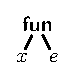
\includegraphics[bb=72 697 93 721]{fun_tree.eps}\\
          $e_1 \;\; e_2$
          & 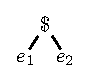
\includegraphics[bb=72 695 101 720]{app_tree.eps}\\
          \bottomrule
        \end{tabular}
      \end{center}
      \smallskip

      \item Note that we needed some symbol for the root of the
        application tree (\texttt{\$}). Traditionally, that symbol is
        (\texttt{@}), but \OCaml uses it already for something else.

      \item When trees represent programs, they are called
        \textbf{abstract syntax trees} (AST).

  \end{itemize}

\end{slide}

\begin{slide}
  \title{Abstract syntax}

  \begin{itemize}

    \item Intuitively, the method for constructing abstract syntax
      trees consists in fully parenthesising the expression.

    \item Each parenthesis corresponds to a subexpression and each
      subexpression corresponds to a subtree.

    \item The tree is built from the root, down to the leaves, by
      traversing subexpressions from the outermost to the innermost,
      that is, the most embedded ones.

    \item For instance, consider
      \begin{center}
        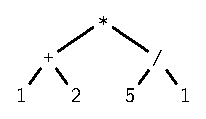
\includegraphics{arith_tree1.eps}
        \qquad
        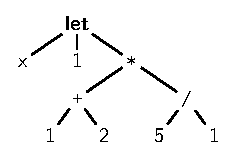
\includegraphics[bb=51 658 175 721]{arith_tree2.eps}
      \end{center}
  \centerline{\texttt{((1+2)*(5/1)) \quad\qquad \texttt{\textbf{let} x = 1 \textbf{in} (1+2)*5/1}}}

  \end{itemize}

\end{slide}

\begin{slide}
  \title{Abstract syntax}

  \begin{itemize}

  \item Another example:
\begin{alltt}
\textbf{let} x = 1 \textbf{in} ((\textbf{let} x = 2 \textbf{in} x) + x)
\end{alltt}
    corresponds to the abstract syntax tree
    \begin{center}
      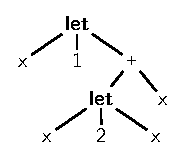
\includegraphics[bb=71 658 160 721]{arith_tree3.eps}
    \end{center}

    \item This example features two local definitions of ``x'': is one
      the redefinition of the other? Is one hiding the other?

    \item There are also two uses of ``x'': which use corresponds to
      which definition?

  \end{itemize}

\end{slide}

\begin{slide}
  \title{Bindings, environments, scope}

  \begin{itemize}

    \item To answer theses questions, we must first understand
      \begin{itemize}

        \item what a \textbf{binding} is,

        \item what the \textbf{scope} of a binding is, and

        \item what an \textbf{environment} is.
      \end{itemize}

    \item The expression we called \textbf{local definition} earlier:
      \begin{equation*}
        \Xlet \;\; x \;\; = \;\; e_1 \;\; \Xin \;\; e_2
      \end{equation*}
      is evaluated as follows:
      \begin{enumerate}

        \item The expression \(e_1\)~is evaluated,

        \item assuming it has a value~\(v_1\), then \(v_1\) is
          \textbf{bound} to the variable~\(x\),

        \item the expression \(e_2\)~is evaluated under the assumption
          that \(x\)~is bound to~\(v_1\).

      \end{enumerate}

  \end{itemize}

\end{slide}

\begin{slide}
  \title{Bindings, environments, scope}

  \begin{itemize}

    \item A local definition
      \begin{equation*}
        \Xlet \;\; x \;\; = \;\; e_1 \;\; \Xin \;\; e_2
      \end{equation*}
      associates the value~\(v_1\) of expression~\(e_1\) to the
      variable denoted by~\(x\), making up a \textbf{binding} noted
      \(x \; \mapsto \; v_1\), and then proceeds to evaluate~\(e_2\)
      with this binding available.

    \item The binding \(x \;\; \mapsto \;\; v_1\) is not usable
      outside the evaluation of~\(e_2\).

    \item We say that the \textbf{scope} of the definition is made of
      the subtrees of the abstract syntax tree corresponding
      to~\(e_2\) where the binding of that definition is usable
      (``visible'').

    \item A mapping from variables to values is called an
      \textbf{environment}.

    \item Let us note \(\rho_\varnothing\) the empty environment.

    \item We write
      \begin{equation*}
        x \;\; \mapsto \;\; v \;\; \oplus \;\; \rho
      \end{equation*}
      to mean that the binding \((x \;\; \mapsto \;\; v)\) was added
      to the environment~\(\rho\).

      %% For example, \([a \mapsto 0; b \mapsto \textbf{fun} \, x
      %%   \rightarrow x]\).

%%    \item We use the same notation for environments as for \OCaml
%%      lists, each new binding being pushed on the left.

    %% \item Note that a binding is a pair made of a variable and a
    %%   value, and we could therefore write it as \((x,v)\), but the
    %%   notation \(x \mapsto v\) explicits the interpretation as a
    %%   binding.

  \end{itemize}

\end{slide}

\begin{slide}
  \title{Bindings, environments, scope}

  \begin{itemize}

    \item Consider again the program
      \smallskip
\begin{alltt}
\textbf{let} x = 0 \textbf{in}
\textbf{let} id = \textbf{fun} x \(\rightarrow\) x \textbf{in}
\textbf{let} y = id x \textbf{in}
\textbf{let} x = (\textbf{fun} x \(\rightarrow\) \textbf{fun} y \(\rightarrow\) x + y) 1 2
\textbf{in} x + 1
\end{alltt}

    \item The variable~\texttt{x} in the expression \texttt{x+1}
      denotes the value of the expression bound to the
      variable~\texttt{x} in the previous line, not the first.

    \item Bindings are ordered in the environment \textbf{by the order
      of their definitions}.

    \item Let us follow the evolution of the environment.

  \end{itemize}

\end{slide}

\begin{slide}
  \title{Bindings, environments, scope}

  \begin{enumerate}

    \item The environment is initially empty: \(\rho_\varnothing\);

    \item \texttt{\textbf{let} x = 0 \textbf{in} \ldots}\\ yields
      $(\ident{x} \;\mapsto\; 0) \oplus \rho_\varnothing$;

    \item \texttt{\textbf{let} id = \textbf{fun} x $\rightarrow$ x
      \textbf{in} \ldots}\\ yields $(\ident{id} \; \mapsto \; \Xfun
      \;\; \ident{x} \rightarrow \ident{x}) \oplus (\ident{x} \;
      \mapsto \; 0) \oplus \rho_\varnothing$;

    \item \texttt{\textbf{let} y = id x \textbf{in} \ldots}\\ yields
      $(\ident{y} \; \mapsto \; 0) \oplus (\ident{id} \; \mapsto \;
      \Xfun \;\; \ident{x} \rightarrow \ident{x}) \oplus (\ident{x} \;
      \mapsto \; 0) \oplus \rho_\varnothing$;

    \item \texttt{\textbf{let} x = \ldots}\\ yields
      $(\underline{\ident{x} \; \mapsto \; 3}) \oplus (\ident{y} \;
      \mapsto \; 0) \oplus (\ident{id} \; \mapsto \; \Xfun \;\;
      \ident{x} \rightarrow \ident{x}) \oplus (\ident{x} \; \mapsto \;
      0) \oplus \rho_\varnothing$.

    \item The expression \textsf{x+1} is evaluated in \(3+1=4\)
      because \(\textsf{x} \; \mapsto \; 3\) (the last binding)
      \textbf{hides} \(\textsf{x} \; \mapsto \; 0\) (the first
      binding).

    \item In other words, the first definition of~\texttt{x} was
      \textbf{out of scope} in \texttt{x+1}.

  \end{enumerate}

\end{slide}

\begin{slide}
  \title{Free variables}

  \begin{itemize}

    %% \item If a variable~\(x\) is not bound to a value in an
    %%   environment~\(\rho\), we say that \(x\)~is \textbf{free}
    %%   in~\(\rho\).

    \item By definition, a variable is \textbf{free} in an expression if
      it is not bound by a \Xlet or a \Xfun.

    \item We can understand this concept on a graphic representation
      of the abstract syntax tree.

    \item From each variable occurrence, we move up, towards the
      root.

    \item If we encounter a \Xlet that binds that variable (in the
      left child), we create an oriented edge from the variable to
      that \Xlet, and we stop: the variable is bound.

    \item Otherwise, if we reach the root (no such \Xlet has been
      found), then the variable is free.

  \end{itemize}

\end{slide}

\begin{slide}
  \title{Free variables}

  \begin{center}
    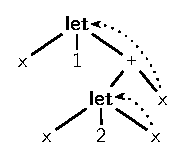
\includegraphics[bb=5 658 169 721]{free_var1.eps}
    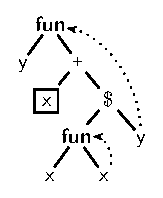
\includegraphics{free_var2.eps}
  \end{center}
  \centerline{\texttt{\textbf{let} x = 1 \textbf{in} ((\textbf{let} x =
      2 \textbf{in} x) + x)} \qquad
        \texttt{\textbf{fun} y \(\rightarrow\) x + (\textbf{fun}
      x \(\rightarrow\) x) y}}

  \begin{itemize}

    \item A similar situation arises with functions: \Xfun is a
      binder, just like \Xlet.

    \item In \Xfun $x \rightarrow e$, the variable~\(x\) (called a
      \textbf{parameter}) may shadow (hide) another variable~\(x\)
      defined on the path to the root.

    \item See above for an example.

    \item We note \(\FV{e}\) the set of the variables free in~\(e\).

  \end{itemize}
\end{slide}

\begin{slide}
  \title{Free variables}

  \begin{itemize}

    \item It is easy to formally define \(\mathcal{F}\) by case and
      recursively:
      \begin{align*}
        \FV{x} &= \{x\}, \quad\texttt{where $x$ is a
          variable}\\
        \FV{c} &= \varnothing, \quad\texttt{where $c$ is a
          constant}\\
        \FV{\Xfun \;\; x \rightarrow e} &=
          \FV{e} \backslash \{x\}\\
          \FV{e_1 \;\; e_2} &= \FV{e_1} \;\cup\; \FV{e_2}\\
          \FV{\Xlet \;\; x \;\; = \;\; e_1 \;\; \Xin \;\; e_2} &=
          \FV{e_1} \;\cup\; \FV{e_2} \backslash \{x\}\\
          \FV{e_1 \;\; \texttt{+} \;\; e_2} &= \FV{e_1} \;\cup\; \FV{e_2}
      \end{align*}

    \item Now, instead of drawing abstract syntax trees, let us use
      these equations to compute the free variables of our previous
      examples.

  \end{itemize}

\end{slide}

\begin{slide}
  \title{Free variables}

  \begin{equation*}
    \begin{array}{lcl}
      \multicolumn{3}{l}{
        \FV{\Xlet \;\; \textsf{x} \;\; = \;\; 1 \;\;
          \Xin \;\; (\Xlet \;\; \textsf{x} \;\; = \;\; 2 \;\;
          \Xin \;\; \textsf{x}) \;\; + \;\; \textsf{x}}} \\
      \phantom{XXX} &=& \FV{1} \;\cup\; \FV{(\Xlet \;\; \textsf{x}
        \;\; = \;\; 2 \;\; \Xin \;\; \textsf{x}) \;\; + \;\;
        \textsf{x}} \backslash \{\textsf{x}\}\\
      \phantom{XXX} &=& \varnothing \;\cup\; (\FV{\Xlet \;\;
        \textsf{x} \;\; = \;\; 2 \;\; \Xin \;\;
        \textsf{x}} \;\cup\; \FV{\textsf{x}}) \backslash \{\textsf{x}\}\\
      \phantom{XXX} &=& (\FV{2} \;\cup\; \FV{\textsf{x}} \backslash
      \{\textsf{x}\}  \;\cup\; \FV{\textsf{x}}) \backslash
      \{\textsf{x}\}\\
      \phantom{XXX} &=& \FV{\textsf{x}} \backslash \{\textsf{x}\}\\
      \phantom{XXX} &=& \varnothing.
    \end{array}
  \end{equation*}

  \bigskip

  \begin{equation*}
    \begin{array}{lcl}
      \multicolumn{3}{l}{ \FV{\Xfun \;\; \textsf{y} \;\; \rightarrow
          \textsf{x} \;\; + \;\; (\Xfun \;\; \textsf{x} \;\;
          \rightarrow \;\; \textsf{x}) \;\; \textsf{y}}}\\ \phantom{X}
      &=& \FV{\textsf{x} + (\Xfun \;\; \textsf{x} \;\; \rightarrow
        \;\; \textsf{x}) \;\; \textsf{y}} \backslash
      \{\textsf{y}\}\\ \phantom{X} &=& (\FV{\textsf{x}} \;\cup\;
      \FV{(\Xfun \;\; \textsf{x} \;\; \rightarrow \;\; \textsf{x})
        \;\; \textsf{y}}) \backslash \{\textsf{y}\}\\ \phantom{X} &=&
      (\{\textsf{x}\} \;\cup\; \FV{\Xfun \;\; \textsf{x} \;\;
        \rightarrow \;\; \textsf{x}} \;\cup\; \FV{\textsf{y}})
      \backslash \{\textsf{y}\}\\ \phantom{X} &=& (\{\textsf{x}\}
      \;\cup\; \FV{\textsf{x}} \backslash \{\textsf{x}\} \;\cup\;
      \{\textsf{y}\}) \backslash \{\textsf{y}\}\\ \phantom{XXX} &=&
      \{\textsf{x}, \textsf{y}\} \backslash
      \{\textsf{y}\}\\ \phantom{X} &=& \{\textsf{x}\}.
    \end{array}
  \end{equation*}

\end{slide}

\begin{slide}
  \title{Closed expressions}

  \begin{itemize}

    \item A \textbf{closed} expression is an expression without free
      variables.

    \item That is, an expression~\(e\) is closed if, and only if,
      \(\FV{e} = \varnothing\).

    \item Only a closed expression can be evaluated (executed).

    \item By extension, we say that~\(e\) is \textbf{closed in an
      environment}~\(\rho\) if \(\FV{e} \subseteq \dom{\rho}\) (the
      free variables are bound in~\(\rho\)).

    \item That is why the first static analysis performed by compilers
      consists in determining the variables which are free in
      expressions: if the program is not closed, it is rejected.

    \item In the case of \texttt{\textbf{fun} y \(\rightarrow\) x +
      (\textbf{fun} x \(\rightarrow\) x) y}, the \OCaml compiler
      prints
      \begin{center}
        \texttt{\textbf{Unbound value x}}
      \end{center}
      and stops. It is useful that this open expression be rejected at
      compile\hyp{}time and does not cause a run\hyp{}time error.

  \end{itemize}

\end{slide}

\begin{slide}
  \title{Evaluation}

  \begin{itemize}

    \item A \textbf{semantics} is a partial function from expressions
      to values. An \textbf{interpreter} or \textbf{evaluator} is a
      program implementing a semantics.

    \item A partial function models the fact that an evaluation may
      not terminate or end in an error.

    \item The \textbf{values} of mini-ML are defined recursively by
      the following cases:\\
      \smallskip
      \begin{tabular}{@{\,}r@{\;\;}ll}
        $\bullet$
        & \emph{unit or integer constant}
        & \unit \ or \textsf{0} or \textsf{1} or \textsf{2}, etc.\\
        $\bullet$
        & \emph{closure}
        & $((\Xfun \;\; x \;\; \rightarrow \;\; e), \, \rho)$,\\
        && where $\rho$ is an environment.\\
%%        && For the operators: $(\lpar{\texttt{+}}\rpar,\rho)$, etc.\\
        $\bullet$
        & \emph{$n$-tuple}
        & $v_1, \dots, v_n$
      \end{tabular}

    \item A \textbf{closure} is a pair made of a function and an
      environment.

    \item That environment is the one at the location where the
      function is defined and the function must be closed in that
      environment (this is called \textbf{static scoping}, or
      \textbf{lexical scoping}).

  \end{itemize}

\end{slide}

\begin{slide}
  \title{Evaluation}

  \begin{itemize}

    \item Let~\(\rho(x)\) be the value most recently bound to~\(x\) in
      the environment~\(\rho\), if any.

    \item We have \((x \;\; \mapsto \;\; v \;\; \oplus \;\; \rho)(x) =
      v\).

    \item We equivalently say that the environment~\(\rho\) was
      \textbf{extended} with the binding \(x \;\; \mapsto \; v\).

    \item The evaluation of an expression must take place in the
      context of an environment, where any free variable must be bound
      (in other words, the expression must be closed in that
      environment).

    \item For example, when evaluating the expression x in
\begin{alltt}
\textbf{let} x = 1 \textbf{in} x
\end{alltt}
      we need the previous environment extended with the binding
      \(\texttt{x} \mapsto 1\).

  \end{itemize}

\end{slide}

\begin{slide}
  \title{Evaluation}

  Let us proceed to define a semantics for our mini-ML, by associating
  to each expression~\(e\) its value~\(v\), assuming the
  environment~\(\rho\):

  \bigskip

  \begin{tabular}{r@{\,\,}ll@{}}
    $\bullet$
  & $x$
  & Look up the \textbf{last} value bound to~\(x\) in~\(\rho\).\\
    $\bullet$
  & $\Xfun \;\; x \;\; \rightarrow \;\; e$
  & The value is $((\Xfun \;\; x \;\; \rightarrow \;\; e), \,\rho)$.\\
    $\bullet$
  & \texttt{+} \ \texttt{-} \ \texttt{/} \ \texttt{*}
  & The value is $(\lpar\texttt{+}\rpar, \,\rho)$, etc.\\
    $\bullet$
  & $e_1$ \texttt{+} $e_2$, etc.
  & Evaluate $e_1$ and $e_2$ in $\rho$, then add, etc.\\
    $\bullet$
  & \unit \ or \textsf{0} or \textsf{1} or \textsf{2}, etc.
  & The value is \unit or \textsf{0} or \textsf{1}, etc.\\
    $\bullet$
  & $\lpar{e}\rpar$
  & Evaluate $e$ into $v$ in $\rho$.\\
    $\bullet$
  & $\Xlet \;\; x \;\; = \;\; e_1 \;\; \Xin \;\; e_2$
  & Evaluate $e_1$ into $v_1$ in $\rho$;\\
  &
  & evaluate $e_2$ into $v$ in $x \;\; \mapsto \; v_1 \;\; \oplus \;\;
    \rho$.\\
    $\bullet$
  & $e_1 \;\; e_2$
  & Evaluate $e_1$ and $e_2$ into $v_1$ and $v_2$ in $\rho$\\
  &
  & (order left unspecified);\\
  &
  & $v_1$ must be of the form $((\Xfun \;\; x \;\; \rightarrow \;\;
    e), \, \rho_1)$;\\
  &
  & evaluate $e$ in $x \;\; \mapsto \; v_2 \;\; \oplus \;\;
    \rho_1$:\\
  && the value is $v$.
\end{tabular}

\end{slide}

\begin{slide}
  \title{Example of evaluation}

  \begin{enumerate}

  \item The environment is initially empty. Let us evaluate
\begin{alltt}
\textbf{let} x = 0 \textbf{in}
\textbf{let} id = \textbf{fun} x \(\rightarrow\) x \textbf{in}
\textbf{let} y = id x \textbf{in}
\textbf{let} x = (\textbf{fun} x \(\rightarrow\) \textbf{fun} y \(\rightarrow\) x + y) 1 2
\textbf{in} x + 1
\end{alltt}

   \item The evaluation of \texttt{\textbf{let} x = 0 \textbf{in}
     \ldots} starts with the evaluation of~\texttt{0}, which,
     obviously, yields~\(0\).

   \item We create the binding $\ident{x} \; \mapsto \; 0$,
     with which we extend~\(\rho_\varnothing\), that is, $\ident{x}
     \;\; \mapsto \; 0 \;\; \oplus \;\; \rho_\varnothing$.

   \item We evaluate the elided subexpression within this new
     environment.

  \end{enumerate}

\end{slide}

\begin{slide}
  \title{Example of evaluation}

  \begin{itemize}

    \item The evaluation of \texttt{\textbf{let} id = \textbf{fun} x
      \(\rightarrow\) x \textbf{in} \ldots} is performed within the
      environment $\ident{x} \;\; \mapsto \;\; 0 \;\; \oplus \;\;
      \rho_\varnothing$.

    \item The value~\(v\) of~\texttt{id} is then the closure $((\Xfun
      \;\; \ident{x} \;\; \rightarrow \;\; \ident{x}), \ident{x} \;\;
      \mapsto \;\; 0 \;\; \oplus \;\; \rho_\varnothing)$.

    \item We extend the current environment with $\ident{id} \;\;
      \mapsto \;\; v$ and we evaluate the elided subexpression with
      it.

    \item The evaluation of \texttt{\textbf{let} y = id x \textbf{in}
      \ldots} is done within the environment $\rho = (\ident{id} \;\;
      \mapsto \;\; ((\Xfun \;\; \ident{x} \;\; \rightarrow \;\;
      \ident{x}), \ident{x} \;\; \mapsto \;\; 0 \;\; \oplus \;\;
      \rho_\varnothing)) \oplus (\ident{x} \;\; \mapsto \; 0) \;\;
      \oplus \;\; \rho_\varnothing$.

    \item We evaluate first (\texttt{id x}) in~\(\rho\).

    \item In order to do so, we evaluate~\texttt{id} and~\texttt{x}
      separately.

    \item These are both variables, thus we look them up in the
      environment to retrieve their last corresponding binding:
      \(\rho(\ident{id}) = ((\Xfun \;\; \ident{x} \rightarrow
      \ident{x}), \ident{x} \mapsto 0 \oplus \rho_\varnothing)\), and
      \(\rho(\texttt{x}) = 0\).

    \item We need to evaluate the body~\texttt{x} in the environment
      $\rho = (\ident{x} \mapsto 0) \oplus (\ident{x} \mapsto 0)
      \oplus \rho_\varnothing$, which yields~\(\rho(\ident{x}) = 0\),
      etc.

  \end{itemize}

\end{slide}

%% \begin{slide}
%%   \title{Example of evaluation}

%%   \begin{itemize}

%%     \item We create the binding $\ident{y} \mapsto 0$, we add it to
%%       the current environment and we evaluate the elided subexpression
%%       with the new environment.

%%     \item The evaluation of \texttt{\textbf{let} x = (\textbf{fun} x
%%       \(\rightarrow\) \textbf{fun} y \(\rightarrow\) x + y) 1 2
%%       \textbf{in} \ldots} uses the environment \([\ident{y} \mapsto 0;
%%       \ident{id} \mapsto ((\Xfun \;\; \ident{x} \rightarrow
%%       \ident{x}), [\ident{x} \mapsto 0]); \ident{x} \mapsto 0]\).


%%     \item Let us stop here and move to expressing the above semantics
%%       in a formal manner.
%%   \end{itemize}

%% \end{slide}

\begin{slide}
  \title{Formal semantics}

  \begin{itemize}

    \item If we note \(\evalf{e}{\rho}\) the value obtained by
      evaluating the expression~\(e\) in the environment~\(\rho\),
      then the evaluation of mini-ML is:
      \begin{align*}
        \evalf{\overline{n}}{\rho} &= n, \;\, \text{with
          $\overline{n}$ an \OCaml integer and $n \in \mathbb{N}$}\\
        \evalf{e_1 \;\; \texttt{+} \;\; e_2}{\rho} &=
        \evalf{e_1}{\rho} \;\; + \;\;
        \evalf{e_2}{\rho} \;\; \in \;\; \mathbb{N}\\
        \evalf{\lpar{e}\rpar}{\rho} &= \evalf{e}{\rho}\\
        \evalf{x}{\rho} &= \rho(x)\\
        \evalf{\Xfun \;\; x \;\; \rightarrow \;\; e}{\rho} &= (\Xfun
        \;\; x \;\; \rightarrow \;\; e), \; \rho\\
        \evalf{e_1 \;\; e_2}{\rho} &= \evalf{e_3}{(x \;\; \mapsto \;\;
          \evalf{e_2}{\rho} \;\; \oplus \;\; \rho_3)},\\
        &\phantom{=\llbracket} \textnormal{where} \ \evalf{e_1}{\rho} =
        (\Xfun \;\; x \;\; \rightarrow \;\; e_3), \, \rho_3\\
        \evalf{\Xlet \;\; x \;\; = \;\; e_1 \;\; \Xin \;\; e_2}{\rho}
        &= \evalf{(\Xfun \;\; x \;\; \rightarrow \;\; e_2) \;\;
          e_1}{\rho}.
      \end{align*}

    \item Note that we write ``$x,\, y$'' instead of ``$(x,\, y)$''
      for brevity.

    \item Evaluation means applying the equations from left to right.

  \end{itemize}

\end{slide}

\begin{slide}
  \title{Partial applications}

  \begin{itemize}

  \item We can easily work out that
      \begin{equation*}
        \evalf{\Xlet \;\; x \;\; = \;\; e_1 \;\; \Xin \;\; e_2}{\rho}
        = \evalf{e_2}{(x \;\; \mapsto \;\; \evalf{e_1}{\rho} \;\;
          \oplus \;\; \rho)}.
      \end{equation*}

    \item Since closures are values, they can be the value of a
      function call:
      \smallskip
\begin{alltt}
\textbf{let} add = \textbf{fun} x \(\rightarrow\) \textbf{fun} y \(\rightarrow\) x + y \textbf{in}
\textbf{let} incr = add 1
\textbf{in} incr 5
\end{alltt}

    \item The call (\texttt{add 1}) is a \textbf{partial application},
      as opposed to a \textbf{complete application} like (\texttt{add 1
        5}).

    \item A partial application, by definition, always evaluates in a
      closure.

    \item Operations are functions denoted by a symbol used in infix
      position (between the operands). As such, they can be partially
      evaluated:
      \smallskip
\begin{alltt}
\textbf{let} incr = (+) 1 \textbf{in} incr 5
\end{alltt}
     \smallskip
     \noindent where the parentheses in~\texttt{(+)} mean that the
     operator has to be considered in \textbf{prefix} position.

  \end{itemize}

\end{slide}

\begin{slide}
  \title{Auto-application and termination}

  \begin{itemize}

    \item Our mini-ML is \textbf{Turing\hyp{}complete}, just as \OCaml
      is.

    \item For instance, we can write the following
      non\hyp{}terminating program:
      \smallskip
\begin{alltt}
\textbf{let} omega = \textbf{fun} f \(\rightarrow\) f f \textbf{in} omega omega
\end{alltt}

    \item The function \texttt{omega} is an
      \textbf{auto\hyp{}applicative function}.

    \item It enables the following non\hyp{}terminating evaluation:
      \smallskip
      \begin{gather*}
        \evalf{\texttt{\textbf{let} omega = \textbf{fun} f \(\rightarrow\) f f \textbf{in} omega omega}}{\rho}\\
\begin{align*}
&= \evalf{\texttt{omega omega}}{(\texttt{omega} \;\; \mapsto \;\;
    \evalf{\texttt{\textbf{fun} f \(\rightarrow\) f f}}{\rho} \oplus
    \rho)}\\ &= \evalf{\texttt{f f}}{(\texttt{\small f} \;\; \mapsto
    \;\; ((\texttt{\textbf{fun} f \(\rightarrow\) f f}), \, \rho)
    \;\; \oplus \;\; \rho)}\\ &= \text{\emph{idem.}}
\end{align*}
\end{gather*}

  \end{itemize}

\end{slide}

\begin{slide}
  \title{Fixed points}

  \begin{itemize}

    \item To demonstrate the expressive power of our mini-ML, let us
      see how we can simulate recursive functions by means of the
      \texttt{omega} function:
      \smallskip
\begin{alltt}
\textbf{let} omega = \textbf{fun} f \(\rightarrow\) f f
\end{alltt}

    \item Let us define a function \texttt{fix}, called the \textbf{Y
      combinator} in \(\lambda\)-calculus:
      \smallskip
\begin{alltt}
\textbf{let} fix = \textbf{fun} g \(\rightarrow\) omega (\textbf{fun} h \(\rightarrow\) \textbf{fun} x \(\rightarrow\) g (h h) x)
\end{alltt}

      \item We can show that, for any function~\(f\),
        \begin{equation*}
          \evalf{f \; \lpar\ident{fix} \; f\rpar{}}{\rho} \;\; = \;\;
          \evalf{\ident{fix} \; f}{\rho}.
        \end{equation*}

      \item In other words, we have
        \begin{equation*}
          f \; \lpar\ident{fix} \; f\rpar
          \;\; \equiv \;\; \ident{fix} \; f.
        \end{equation*}

      \item The fixed point~\(x\) of a (continuous) function~\(g\)
        satisfies \(g(x) = x\).

      \item Therefore, the fixed point of~\ident{f} (if it exists) is
        the value of \lpar\ident{fix} \ident{f}\rpar{}.

  \end{itemize}

\end{slide}

\begin{slide}
  \title{Fixed points}

  \begin{itemize}

    %% \item Just as with \Xlet \Xin, we can simplify the semantics of
    %%   \texttt{fix}:
    %%   \begin{equation*}
    %%     \evalf{\ident{fix} \;\; e}{\rho} = \evalf{e_1}{(f \mapsto
    %%       \evalf{\ident{fix} \, \lpar\Xfun \, f \rightarrow
    %%         e_1\rpar}{\rho} \oplus \rho_1)},
    %%   \end{equation*}
    %%   where $\evalf{e}{\rho} = (\Xfun \, f \rightarrow e_1), \, \rho_1$.

    \item Let us consider the following definitions:
    \smallskip
\begin{alltt}
\textbf{let} pre\_fact =
\ \ \textbf{fun} f \(\rightarrow\) \textbf{fun} n \(\rightarrow\) \textbf{if} n = 1 \textbf{then} 1 \textbf{else} n * f(n-1)
\textbf{let} fact = fix pre\_fact
\end{alltt}

    \item We see that \texttt{fact} is the fixed point of
      \texttt{pre\_fact}:
      \smallskip
      \begin{align*}
        \evalf{\texttt{fact}}{\rho} &= \evalf{\texttt{fix
            pre\_fact}}{\rho}\\
        &= \evalf{\texttt{pre\_fact (fix pre\_fact)}}{\rho}\\
        &= \evalf{\texttt{pre\_fact fact}}{\rho}\\
        &= \evalf{\texttt{\textbf{fun} n \(\rightarrow\) \textbf{if} n
            = 1 \textbf{then} 1 \textbf{else} n * fact(n-1)}}{\rho}
      \end{align*}

    \item It is as if the definition of ``\texttt{fact}'' were
      recursive... but it is not.

  \end{itemize}

\end{slide}

\begin{slide}
  \title{Local recursive definitions}

  \begin{itemize}

    \item The function ``\texttt{fact}'' coincides pointwise with the
      factorial function.

    %% \item We could then predefine the fixed point operator
    %%   ``\texttt{fix}'' (not necessarily the one we used above) and
    %%   allow the programmer to use it directly.

    \item Let us extend mini-ML with a native recursive binder, using
      the ``\texttt{fix}'' function:
      \smallskip
      \begin{equation*}
        \evalf{\Xlet \;\; \Xrec \;\; f \;\; = \;\; e_1 \;\; \Xin \;\;
          e_2}{\rho} \;\; = \;\; \evalf{\Xlet \;\; f \;\; = \;\;
          \textsf{fix} \; \lpar\Xfun \;\; f \;\; \rightarrow \;\; e_1\rpar \;\;
          \Xin \;\; e_2}{\rho}.
      \end{equation*}

  \end{itemize}

\end{slide}

\begin{slide}
  \title{Extensions}

  \begin{itemize}

    \item Let us extend our mini-ML with the following
      expressions.\\
      \smallskip
      \begin{tabular}{r@{\,\,}ll@{}}
        $\bullet$
        & \emph{Boolean constants}
        & \Xtrue{} or \Xfalse\\
        $\bullet$
        & \emph{Boolean operators}
        & \texttt{(\&\&)} or \texttt{(||)} or \textsf{\textbf{not}}\\
        $\bullet$
        & \emph{$n$-tuple}
        & $e_1, \ldots, e_n$\\
        $\bullet$
        & \emph{conditional}
        & \Xif{} $e_0$ \Xthen{} $e_1$ \Xelse{} $e_2$\\
        $\bullet$
        & \emph{local recursive binding}
        & \Xlet{} \Xrec{} $f \;\; = \;\; e_1$ \Xin{} $e_2$
      \end{tabular}

      \item Note that parentheses are recommended around tuples, but
        are not mandatory.

      \item Let us distinguish the variables occurring after \Xlet{}
        and \Xfun{}, because they are \textbf{irrefutable patterns},
        noted $\ipat{p}$:\\
        \smallskip
        \begin{tabular}{r@{\,\,}ll@{}}
          $\bullet$
          & \emph{function}
          & $\Xfun \;\; \ipat{p} \rightarrow e$\\
          $\bullet$
          & \emph{local definition}
          & \(\Xlet \;\; \textrm{[}\Xrec\textrm{]} \;\; \ipat{p} \;\;
          = \;\; e_1 \;\; \Xin \;\; e_2\)
        \end{tabular}

  \end{itemize}

\end{slide}

\begin{slide}
  \title{Irrefutable patterns}

  \begin{itemize}

    \item An irrefutable pattern $\ipat{p}$ is defined recursively by
      the following cases:\\
      \smallskip
      \begin{tabular}{r@{\,\,}ll@{}}
        $\bullet$
        & \emph{variable}
        & $f, g, h, x, y, z$, etc. \\
        $\bullet$
        & \emph{unit}
        & \unit\\
        $\bullet$
        & \emph{$n$-tuple}
        & $\ipat{p}_1, \ldots, \ipat{p}_n$\\
        $\bullet$
        & \emph{parenthesis}
        & $\lpar\ipat{p}\rpar$\\
        $\bullet$
        & \emph{underscore}
        & {\Large \_}
      \end{tabular}

      \item Note that, from the syntactic point of view, irrefutable
        patterns are special cases of expressions, except the
        underscore, which is a special case avoiding the creation of a
        binding.

      \item The sentence~\(e\) is equivalent to \(\Xlet \;\; \_ \;\; =
        \;\; e\).

  \end{itemize}

\end{slide}

\begin{slide}
  \title{Extensions}

  \begin{itemize}

    \item The comma takes priority over the arrow:
      \begin{equation*}
        \Xfun \;\; x \;\;
        \rightarrow \;\; x, \, y \;\; = \;\;
        \Xfun \;\; x \;\; \rightarrow \;\; (x,\,y).
      \end{equation*}

    \item In order to alleviate the notation $\Xfun \;\; \ipat{p}_1
      \;\; \rightarrow \;\; \ldots \;\; \rightarrow \;\; \Xfun \;\;
      \ipat{p}_n \;\; \rightarrow \;\; e$, we define the equivalent
      expressions:\\
      \smallskip
      \begin{tabular}{r@{\,\,}ll@{}}
        $\bullet$
        & $\Xlet \;\;
          \textrm{[}\Xrec\textrm{]} \;\; f \;\;\;
          = \;\; \Xfun \;\; \ipat{p}_1 \;\; \ipat{p}_2 \;\; \ldots \;\;
          \ipat{p}_n \;\; \rightarrow \;\; e$
        & (new expression)\\
        $\bullet$
        & $\Xlet \;\;
          \textrm{[}\Xrec\textrm{]} \;\; f
          \;\;\; \ipat{p}_1 \;\; \ipat{p}_2 \;\; \ldots \;\; \ipat{p}_n
          \;\; = \;\; e$
        & (new sentence)
      \end{tabular}

    \item For example, we would write
\begin{alltt}
\textbf{let} mult = \textbf{fun} x y \(\rightarrow\) x * y \textbf{in}
\textbf{let} eq x y = (x = y) \textbf{in}
\textbf{let rec} fact n = \textbf{if} eq n 1 \textbf{then} 1 \textbf{else} mult n (fact(n-1))
\textbf{in} fact 9
\end{alltt}

      \item Note the two different meanings of \texttt{(=)}: one is
        definitional, the other is operational (a Boolean operator).

  \end{itemize}

\end{slide}

\begin{slide}
  \title{Parallel definitions}

  \begin{itemize}

    \item We also extend the syntax to alleviate certain
      expressions. By definition,
      \begin{equation*}
        \Xlet \;\; \ipat{p}_1 \;\; = \;\; e_1 \;\;
        \Xand \;\; \ipat{p}_2 \;\; = \;\; e_2 \;\; \ldots \;\;
        \Xand \;\; \ipat{p}_n \;\; = \;\; e_n \;\; \Xin \;\; e
      \end{equation*}
      is equivalent to
      \begin{equation*}
        \Xlet \;\; \ipat{p}_1, \ldots, \ipat{p}_n \;\; = \;\; e_1,
        \ldots, e_n \;\; \Xin \;\; e
      \end{equation*}
      but the latter requires more memory (for the tuples in the heap).

    \item These are called \textbf{parallel definitions} because they
      occur within the same environment and could be conceived as
      happening in parallel.

    \item The two following sentences are equivalent:
      \smallskip
\begin{alltt}
\textbf{let} x = 1 \textbf{and} y = 2 \textbf{in} x + y
\textbf{let} x,y = 1,2 \textbf{in} x + y
\end{alltt}

  \end{itemize}

\end{slide}

\begin{slide}
  \title{Mutually recursive definitions}

  \begin{itemize}

    \item Parallel definitions are useful for \textbf{mutually
      recursive definitions}:\\
      \smallskip
      \begin{tabular}{r@{\;}ll}
        $\bullet$
        & \(\Xlet \;\; \Xrec \;\; \ipat{p}_1 \;\; = \;\; e_1 \;\;
        \Xand \;\; \ipat{p}_2 \;\; = \;\; e_2 \; \ldots \;\; \Xand
        \;\; \ipat{p}_n \;\; = \;\; e_n \;\; \Xin \;\; e\) &
        (expression)\\
      $\bullet$
      & \(\Xlet \;\; \Xrec \;\; \ipat{p}_1 \;\; = \;\; e_1 \;\; \Xand
        \;\; \ipat{p}_2 \;\; = \;\; e_2 \; \ldots \;\; \Xand \;\;
        \ipat{p}_n \;\; = \;\; e_n\)
      & (sentence)
      \end{tabular}
      \smallskip

    \item A silly example:
      \smallskip
\begin{alltt}
\textbf{let} \textbf{rec} even n = \textbf{if} 2*(n/2) = n \textbf{then} true \textbf{else} odd (n-1)
\textbf{and} odd n = \textbf{if} 2*(n/2) = n \textbf{then} false \textbf{else} even (n-1)
\end{alltt}
     \smallskip
     \noindent where \texttt{(/)} is the Euclidean division.

  \end{itemize}

\end{slide}

\begin{slide}
  \title{Mutually recursive definitions}

  \begin{itemize}

    \item Let us consider the case where the irrefutable patterns are
      variables:
      \begin{equation*}
        \Xlet \;\; x \;\; = \;\; e_1 \;\; \Xand \;\; y \;\; = \;\; e_2
        \;\; \Xin \;\; e
      \end{equation*}
      where $x \neq y$.

    \item If~\(x\) is not free in~\(e_2\), i.e., $x \not\in
      \FV{e_2}$, then the previous construct is equivalent to \[\Xlet
      \;\; x \;\; = \;\; e_1 \;\; \Xin \;\; \Xlet \;\; y \;\; = \;\;
      e_2 \;\; \Xin \;\; e.\]

    \item If~\(x\) is free in~\(e_2\), that is, $x \in \FV{e_2}$, then
      the previous construct is defined as being equivalent to
      \begin{center}
        \begin{minipage}{0.3\linewidth}
          \begin{tabbing}
            \underline{\Xlet} \= \underline{$z$ \equal{} $x$ \Xin}\\
            \> \Xlet{} $x$ \equal{} $e_1$ \Xin\\
            \> \Xlet{} $y$ \equal{} \underline{\Xlet{} $x$ \equal{}
              $z$ \Xin} $e_2$\\
            \Xin $e$
          \end{tabbing}
        \end{minipage}
      \end{center}
      where \(z \not\in \FV{e_1} \;\cup\; \FV{e_2} \;\cup\; \FV{e}\),
      in order to avoid being captured by~\(e_1\), \(e_2\)~or~\(e\).

%    \item It is thus not an elementary construct.

  \end{itemize}

\end{slide}

\begin{slide}
  \title{Mutually recursive definitions}

  \begin{itemize}

    \item The parallel \Xlet{} \Xrec{} (with \Xand) can always be
      reduced to a simple \Xlet{} \Xrec{} (with \Xin) by
      parameterising one of the definitions by the other.

    \item Consider the following sentence
      \begin{equation*}
        \Xlet \;\; \Xrec \;\; x \;\; = \;\; e_1 \;\; \Xand \;\; y \;\;
        = \;\; e_2 \;\; \Xin \;\; e
      \end{equation*}
      where $x \neq y$.

    \item It is equivalent, by definition, to
      \begin{center}
        \begin{minipage}{0.3\linewidth}
          \begin{tabbing}
            \Xlet{} \= \Xrec{} $x$ \equal{} \underline{\Xfun{} $y$
              $\rightarrow$} $e_1$ \Xin\\
            \> \Xlet{} \Xrec{} $y$ \equal{} \underline{\Xlet{} $x$
              \equal{} $x \;\; y$ \Xin} $e_2$ \Xin\\
            \> \underline{\Xlet{} $x$ \equal{} $x \;\; y$}\\
            \underline{\Xin} $e$
          \end{tabbing}
        \end{minipage}
      \end{center}

    \item Note how ($x$ $y$) is evaluated twice.

  \end{itemize}

\end{slide}

\begin{slide}
  \title{Static typing and inference}

  \begin{itemize}

    \item The aim of \textbf{static typing} is to detect and reject at
      compile\hyp{}time some kinds of programming errors which would
      otherwise result into an error at run\hyp{}time, like \texttt{(1
        2)} or \texttt{(\textbf{fun} x $\rightarrow$ x) + 1}.

    \item With this aim, a \textbf{type} is assigned by the compiler
      or the programmer to each subexpression of an expression (in
      particular, the whole program).

    \item For example, \type{int} for an arithmetic expression, or
      $\type{int} \rightarrow \type{int}$ for a function from the
      integers to the integers.

    \item The \textbf{coherence} of these types is checked by the
      \OCaml compiler, that is, if we think of a type as an
      assumption, no assumption must contradict another one.

  \end{itemize}

\end{slide}

\begin{slide}
  \title{Static typing and inference}

  \begin{itemize}

    \item It is undecidable to determine all possible run\hyp{}time
      errors for all programs before running them.

    \item \textbf{Type systems}, on the other hand, are often
      \textbf{decidable}, because it is considered a good design to
      ensure that the compiler terminates on all input programs.

    \item Therefore, it is impossible for the compiler to reject only
      those programs that would ``go wrong'' at run\hyp{}time.

    \item In other words, all type systems reject innocent programs,
      and that is why the quest for better type systems, with better
      compromises between unfair rejection and guaranteed safety, will
      never end.

  \end{itemize}

\end{slide}

\begin{slide}
  \title{Types}

  \begin{itemize}

    \item \textbf{Types are terms} associated to expressions, either
      by the programmer or the compiler, and they capture some
      \textbf{invariant properties} which can be automatically
      composed and checked.

    \item A type~$t$ is a term defined recursively by the following
      cases:\\
      \smallskip
      \begin{tabular}{r@{\,\,}ll}
        $\bullet$
        & \emph{simple}
        & \textsf{char}, \textsf{bool}, \textsf{int}, \textsf{string},
        \textsf{float}, \textsf{unit}\\
        $\bullet$
        & \emph{Cartesian product}
        & $t_1 \times \ldots \times t_n$\\
        $\bullet$
        & \emph{functional}
        & $t_1 \rightarrow t_2$\\
        $\bullet$
        & \emph{parenthesis}
        & $(t)$\\
        $\bullet$
        & \emph{free variable}
        & $\alpha$, $\beta$, $\gamma$, etc. \\
        $\bullet$
        & \emph{parameterised}
        & $\alpha$ \textsf{list}
      \end{tabular}

    \item Until now, we have not encountered values of the type
      \textsf{float}, \textsf{char} or \textsf{string}, but they are
      fairly obvious.

    \item We write $\times$, $\alpha$, $\beta$, etc. what is written
      \texttt{*}, \texttt{'a}, \texttt{'b}, etc. in the source code.

  \end{itemize}

\end{slide}

\begin{slide}
  \title{Type expressions}

  \begin{itemize}

    \item The Cartesian product takes multiple arguments, instead of
      being binary like in mathematics, and $(\times)$~is not
      associative in \OCaml:
      \begin{equation*}
        t_1 \times t_2 \times t_3 \;\; \neq \;\; (t_1 \times t_2) \times
        t_3 \;\; \neq \;\; t_1 \times (t_2 \times t_3).
      \end{equation*}

    \item The arrow is used in types too, where it is also
      right\hyp{}associative:
      \begin{equation*}
        t_1 \;\; \rightarrow \;\; t_2 \;\; \rightarrow \;\; \ldots
        \;\; \rightarrow \;\; t_{n-1} \;\; \rightarrow \;\; t_n
      \end{equation*}
      is equivalent to
      \begin{equation*}
        t_1 \;\; \rightarrow \;\; (t_2 \;\; \rightarrow \;\; (\ldots
        (t_{n-1} \;\; \rightarrow \;\; t_n)) \; \ldots).
      \end{equation*}

    \item The Cartesian product has priority over the arrow:
      \begin{equation*}
        t_1 \times t_2 \;\; \rightarrow \;\; t_3
      \end{equation*}
      is equivalent to
      \begin{equation*}
        (t_1 \times t_2) \;\; \rightarrow \;\; t_3.
      \end{equation*}

  \end{itemize}

\end{slide}

\begin{slide}
  \title{Type expressions}

  \begin{itemize}

    \item The \OCaml compiler computes a type for each expression:
      this is called \textbf{static type inference}.

    \item For the simple constants, we have
      \smallskip
      \begin{center}
        \begin{tabular}{l|l|c}
          \toprule
          \multicolumn{1}{c}{Type} & \multicolumn{1}{c}{Values}
          & \multicolumn{1}{c}{Some functions}\\
          \midrule
          \textsf{unit}
          & \unit
          & \\
          \textsf{bool}
          & \Xtrue \ \Xfalse
          & \texttt{\&\&} \ \texttt{||} \ \texttt{not} \\
          \textsf{int}
          & \textsf{1} \, \textsf{2} \ \textsf{max\_int}, etc.
          & \texttt{+} \ \texttt{-} \ \texttt{*} \ \texttt{/}, etc.\\
          \textsf{float}
          & \textsf{1.0} \, \textsf{2.} \ \textsf{1e4}, etc.
          & \texttt{+.} \ \texttt{-.} \ \texttt{*.} \ \texttt{/.} \
          \texttt{cos}, etc.\\
          \textsf{char}
          & \textsf{'a'} \ \textsf{'}\verb+\+\textsf{n'} \
          \textsf{'}\verb+\+\textsf{097'}, etc.
          & \textsf{Char.code} \, \textsf{Char.chr}, etc.\\
          \textsf{string}
          & \textsf{"a}\verb+\+\textsf{tb}\verb+\+\textsf{010c}\verb+\+\textsf{n"},
          etc.
          & \verb+(^)+ \, \textsf{s.[i]}, etc.\\
          \bottomrule
        \end{tabular}
      \end{center}
      \smallskip

    \item Operations on floating point numbers are written differently
      from their equivalent counterparts on integers.
  \end{itemize}

\end{slide}

\begin{slide}
  \title{Type definitions}

  \begin{itemize}

    \item We further extend the syntax of the sentences to allow the
      binding of a type to a name, or \textbf{type definition}:\\
      \smallskip
      \begin{tabular}{@{\,}r@{\,\,}l@{\,\;}l@{}}
        $\bullet$
        & \emph{type definition}
        & \(\textbf{type} \;\; \textrm{[}\textbf{nonrec}\textrm{]}
        \;\; q \;\; = \;\; t\)\\
        $\bullet$
        & \emph{parallel type definition}
        & \(\textbf{type} \;\; \textrm{[}\textbf{nonrec}\textrm{]}
        \;\; q_1 \;\; = \;\; t_1 \;\; \textrm{[}\Xand \;\; q_2 \;\; =
          \;\; t_2 \;\; \ldots\textrm{]}\)\\
        $\bullet$
        & \emph{type variable}
        & $q$\\
        \multicolumn{2}{l}{In particular:}\\
        $\bullet$
        & \emph{type aliasing}
        & \(\textbf{type} \;\; q_0 \;\; = \;\; q_1\)
      \end{tabular}
      \smallskip

    \item By default, type definitions can be recursive (we will see
      an example later). If not, use the keyword \textbf{nonrec}.

    \item \noindent We can now write, for instance, the following:
\begin{alltt}
\textbf{type} abscissa = float
\textbf{type} ordinate = float
\textbf{type} point = abscissa \(\times\) ordinate
\textbf{type} origin = point
\end{alltt}

  \end{itemize}

\end{slide}

\begin{slide}
  \title{Type inference}

  \begin{itemize}

    \item Tuples contain data of the same type and their arity is part
      of their type.

    \item For instance, the pair \textsf{(1,2)} has type \textsf{int}
      $\times$ \textsf{int}, and the triplet \textsf{(1,2,3)} has type
      \textsf{int} $\times$ \textsf{int} $\times$ \textsf{int}, thus
      are incompatible.

    \item Consider also the following session at the \OCaml
      toplevel:
      \medskip

      \noindent\topin{\textbf{let} middle x y = (x+y)/2}

      \noindent\topout{\textbf{val} middle~:~int $\rightarrow$ int
        $\rightarrow$ int}

      \medskip

      \noindent\topin{\textbf{let} middle (x,y) = (x+y)/2}

      \noindent\topout{\textbf{val} middle~:~int $\times$ int
        $\rightarrow$ int}

      \smallskip

    \item In the above, the \OCaml compiler figures out in both cases
      that, since we compute \texttt{(x+y)}, that implies that
      \texttt{x}~and~\texttt{y} must have type \type{int}.
  \end{itemize}

\end{slide}

\begin{slide}
  \title{Polymorphism}

  \begin{itemize}

    \item When a variable is not constrained by its uses,
      like~\texttt{x} in \texttt{(\textbf{fun} x $\rightarrow$ x)}, it
      is assigned the most general type, that is, a \textbf{type
        variable}:\\
      \noindent\topin{\textbf{let} id = \textbf{fun} x $\rightarrow$
        x}

      \noindent\topout{\textbf{val} id : $\alpha \rightarrow \alpha =
        \topclos$}

    \item This means that the above identity function can be applied
      to any kind of value, and that the type of the call is that of
      the argument.

    \item This property of a function to accept values of different
      types is called \textbf{parametric polymorphism}. Consider more
      examples:\\
      \noindent\topin{\textbf{fun} (x,y,z) $\rightarrow$ x}

      \noindent\topout{\textbf{-} : $\alpha \times \beta \times
        \gamma \rightarrow \alpha$}.

      \noindent\topin{\textbf{let} compose f g = \textbf{fun} x
        \(\rightarrow\) f (g x)}

      \noindent\topout{\textbf{val} compose~: $(\alpha \rightarrow
        \beta) \rightarrow (\gamma \rightarrow \alpha) \rightarrow
        \gamma \rightarrow \beta = \topclos$}
\begin{alltt}
\textbf{\# let rec} power f n =
\ \ \ \ \textbf{if} n \(\leqslant\) 0 \textbf{then} id \textbf{else} compose f (power f (n-1));;
\end{alltt}
      \noindent\topout{\textbf{val} power~:~($\alpha \rightarrow \alpha$)
        $\rightarrow$ int $\rightarrow$ ($\alpha \rightarrow \alpha$) =
        $\topclos$}

  \end{itemize}

\end{slide}

\begin{slide}
  \title{Polymorphism inference}

  \noindent\topin{\textbf{let} compose f g = \textbf{fun} x
    \(\rightarrow\) f (g x)}

  \noindent\topout{\textbf{val} compose~: $(\alpha \rightarrow \beta)
    \rightarrow (\gamma \rightarrow \alpha) \rightarrow \gamma
    \rightarrow \beta = \topclos$}

  \bigskip

  The type of the function \fun{compose} is inferred as follows:
  \begin{itemize}

    \item the first argument~\textsf{f} is an arbitrary function,
      hence of type \(\alpha \rightarrow \beta\);

    \item the second argument~\textsf{g} is a function whose result is
      the argument of~\textsf{f}, therefore of type~\(\alpha\);

    \item the domain of~\textsf{g} is arbitrary, hence \textsf{g}~has
      type \(\gamma \rightarrow \alpha\);

    \item the function \fun{compose} has an argument~\textsf{x}
      which is passed to~\textsf{g}, hence has type~\(\gamma\);

    \item finally, the result of \fun{compose} is returned
      by~\textsf{f}, hence of type~\(\beta\).

  \end{itemize}

\end{slide}

\begin{slide}
  \title{Polymorphic equality}

  \begin{itemize}

    \item The \textbf{equality operator} in \OCaml is polymorphic and
      built in:

      \smallskip
      \noindent\topin{(=)}

      \noindent\topout{- : $\alpha \rightarrow \alpha \rightarrow
        \texttt{bool} = \topclos$}

      \item We must be very careful that it coincides with our
        intended notion of equality, because the compiler will always
        accept it on \textbf{non\hyp{}functional values}.

      \item It consists in the \textbf{syntactical equality}: two
        values are equal if they have the same structure and if their
        respective parts are equal, recursively. It fails on closures.

        \smallskip

        \noindent\topin{1 = 1 \&\& [1;2] = [1;2] \&\& \str{yes} =
          \str{yes}}

        \noindent\topout{- : bool = true}

        \noindent\topin{(\textbf{fun} x \(\rightarrow\) x) =
          (\textbf{fun} x \(\rightarrow\) x)}

        \error{Exception: Invalid\_argument "equal: functional value".}

  \end{itemize}

\end{slide}

\begin{slide}
  \title{Pattern matching}

  \begin{itemize}

    \item Let us extend expressions with \textbf{matching} a value
      against \textbf{patterns}. Let~$p_i$ be patterns in
      \begin{center}
        \Xmatch{} $e$ \Xwith{} $p_1 \; \rightarrow \; e_1 \; \mid \;
        \ldots \; \mid \; p_n \; \rightarrow \; e_n$.
      \end{center}

    \item Patterns are recursively defined by the following cases:\\
      \smallskip
      \begin{tabular}{r@{\,\,}ll}
        $\bullet$
        & \emph{variable}
        & $f, g, h$ (functions) and $x, y, z$ (others). \\
        $\bullet$
        & \emph{unit or constant}
        & \unit \ or \textsf{0} or \Xtrue{}, etc.\\
        $\bullet$
        & \emph{$n$-tuple}
        & $p_1, \ldots, p_n$\\
        $\bullet$
        & \emph{parenthesis}
        & $\lpar{p}\rpar$\\
        $\bullet$
        & \emph{underscore}
        & {\Large \_}
      \end{tabular}

    \item Note that irrefutable patterns are patterns.

    \item \textbf{Pattern matching} is used to define functions case
      by case:
\begin{alltt}
\textbf{let rec} fib n =
\ \ \textbf{match} n \textbf{with}
\ \ \ \ 0 \(\rightarrow\) 1
\ \ | 1 \(\rightarrow\) 1
\ \ | \_ \(\rightarrow\) fib(n-1) + fib(n-2)
\end{alltt}

  \end{itemize}

\end{slide}

\begin{slide}
  \title{Pattern matching}

  \begin{itemize}

    \item As in mathematics, the order of the cases is that of the
      writing, and the previous definition reads like so:
      \begin{quote}
        If the value of~\texttt{n} has the shape~\texttt{0}, then
        \texttt{fib(n)} has the value~\texttt{1}; else, if the value
        of~\texttt{n} has the shape~\texttt{1}, then \texttt{fib(n)}
        has the value~\texttt{1}; for any other value of~\texttt{n},
        \texttt{fib(n)} has the value of \texttt{fib(n-1) + fib(n-2)}.
      \end{quote}

    \item What is the meaning of the relation ``The value~\(v\) has
      the shape~\(p\)''? Or, equivalently: ``The pattern~\(p\) matches
      the value~\(v\)''?

    \item A constant, including \unit, has the shape of itself in a
      pattern (constants are both values and patterns).

    \item A \(n\)-tuple (value) has the shape of a \(n\)-tuple in a
      pattern.

    \item Any value has the shape of a variable in a pattern or of the
      underscore `{\Large \_}'.

  \end{itemize}

\end{slide}

\begin{slide}
  \title{Pattern matching}

  \begin{itemize}

    \item Note that patterns do not match closures, which means that
      the~\(e\) in ``\Xmatch{} $e$ \Xwith{}'' must not have a closure
      as a value. In the case of constants, including \unit, matching
      coincides with equality.

    \item Matching is the evaluation of a \Xmatch expression.

    \item Informally, the evaluation of
      \begin{center}
        \Xmatch{} $e$ \Xwith{} $p_1 \; \rightarrow \; e_1 \; \mid \;
        \ldots \; \mid \; p_n \; \rightarrow \; e_n$
      \end{center}
      begins with that of~$e$ into~$v$.

    \item Next, \(v\)~is compared to the patterns~\(p_i\) for
      increasing values of~\(i\).

    \item If~\(p_i\) is the first pattern to match~\(v\), then the
      value of the matching is the value of~\(e_i\).

    \item Here is a definition of the logical disjunction:
\begin{alltt}
\textbf{let} disj (x,y) = \textbf{match} x,y \textbf{with}
                      \textbf{false}, \textbf{false} \(\rightarrow\) \textbf{false}
                    | \_ \(\rightarrow\) \textbf{true}
\end{alltt}

  \end{itemize}

\end{slide}

\begin{slide}
  \title{Variant types}

  \begin{itemize}

    \item \textbf{Variant types} are a generalisation of
      enumerations.

    \item For instance, Boolean values can be (re)defined as
\begin{alltt}
\textbf{type} boolean = True | False
\textbf{let} true' = True \textbf{and} false' = False
\end{alltt}

    \item Note that \textbf{value constructors}, like \texttt{True} or
      \texttt{False}, must begin with an uppercase letter.

    \item Pattern matching examines the values of a variant type:
\begin{alltt}
\textbf{let} int\_of\_boolean b = \textbf{match} b \textbf{with} True  \(\rightarrow\) 1 | False \(\rightarrow\) 0
\end{alltt}

    \item Value constructors can also carry information beyond their
      mere name. For instance, a pack of playing cards can be defined
      as
\begin{alltt}
\textbf{type} suit = Heart | Diamond | Spade | Club
\textbf{type} face = Ace | King | Queen | Jack | Simple \textbf{of} int
\textbf{type} ordinary = suit \(\times\) face
\textbf{type} card = Card \textbf{of} ordinary | Joker
\end{alltt}

  \end{itemize}

\end{slide}

\begin{slide}
  \title{Variant types}

  Let us define the cards and the functions creating them:
  \medskip

  \noindent\topin{\textbf{let} jack\_of\_spade = Card (Spade, Jack)}

  \noindent\topout{\textbf{val} jack\_of\_spade : card = Card (Spade,
    Jack)}

  \medskip

  \noindent\topin{\textbf{let} card f c = Card (c,f)}

  \noindent\topout{\textbf{val} card : face $\rightarrow$ suit
    $\rightarrow$ card = $\topclos$}

  \medskip

  \noindent\topin{\textbf{let} king = card King}

  \noindent\topout{\textbf{val} king : suit $\rightarrow$ card =
    $\topclos$}

\begin{alltt}
\textbf{\# let} value c =
    \textbf{match} c \textbf{with}
      Card Ace         \(\rightarrow\) 14
    | Card King        \(\rightarrow\) 13
    | Card Queen       \(\rightarrow\) 12
    | Card Jack        \(\rightarrow\) 11
    | Card (Simple k) \(\rightarrow\) k
    | Joker             \(\rightarrow\) 0;;
\end{alltt}

\end{slide}

\begin{slide}
  \title{Pattern matching (resumed)}

  \begin{itemize}

    \item A pattern can capture several cases at once with an
      \textbf{underscore}:
\begin{alltt}
\textbf{let} is\_simple c =
\ \ \textbf{match} c \textbf{with}
\ \ \ \ Card (Simple \_) \(\rightarrow\) \textbf{true}
\ \ | \_ \(\rightarrow\) \textbf{false}
\end{alltt}

    \item A pattern matching is incomplete if there exists at least a
      value which cannot be matched by any pattern.

    \item In that case, a warning is printed at compile\hyp{}time
      because it is strongly advised to \textbf{avoid incomplete
        pattern matchings}:
      \medskip

      \noindent\topin{\textbf{let} simple c = \textbf{match} c
        \textbf{with} Card (\_, Simple k) $\rightarrow$ k}

      \noindent\error{Characters 15-51}

      \noindent\error{Warning: this pattern-matching is not exhaustive.}

      \noindent\error{Here is an example of a value that is not
        matched: Joker}

      \noindent\topout{\textbf{val} simple : card $\rightarrow$ int =
        $\topclos$}

  \end{itemize}

\end{slide}

\begin{slide}
  \title{Pattern matching (resumed)}

  \begin{itemize}

    \item A variable cannot occur twice or more in the same pattern,
      because this requires to call the polymorphic equality during
      pattern matching, which may be costly and even loop on circular
      values (and we want compilers to terminate).

    \item Such a pattern is said to be \textbf{non\hyp{}linear}. (We
      have seen these in the context of rewrite systems.)
      \medskip

      \noindent\topin{\textbf{fun} (x,y) $\rightarrow$ \textbf{match}
        x,y \textbf{with} Card z, z $\rightarrow$ \textbf{true}}

      \noindent\error{Characters 40-41}

      \noindent\error{This variable z is bound several times in this
        matching.}

  \end{itemize}

\end{slide}

\begin{slide}
  \title{Lists}

  \begin{itemize}

    \item Lists can be defined as a polymorphic, \textbf{recursive
      variant type}:
      \smallskip
\begin{alltt}
\textbf{type} \(\alpha\) list' = Nil | Cons \textbf{of} \(\alpha\) \(\times\) \(\alpha\) list'
\end{alltt}

    \item The value constructors \texttt{Nil} and \texttt{Cons} are
      traditional in the community of functional languages. The former
      denotes the empty list; the latter represents a non\hyp{}empty
      list.

    \item We used the same naming in the context of rewrite systems.

    \item A non\hyp{}empty list is then modelled as a pair whose first
      component is an element (of type~\(\alpha\)) of the list and the
      second component is the remainder of the list, or a sublist (of
      type \(\alpha\)~\texttt{list'}). For instance:
      \smallskip
\begin{alltt}
\textbf{let} empty = Nil
\textbf{let} single\_char = Cons ('a', empty)
\textbf{let} single\_int = Cons (4, empty)
\textbf{let} long = Cons (1, Cons (2, Cons (3, single\_int)))
\end{alltt}

  \end{itemize}

\end{slide}

\begin{slide}
  \title{Lists}

  \begin{itemize}

    \item By default, the \OCaml system predefines a type
      \(\alpha\)~\texttt{list}, whose constructor for the empty list
      is~\texttt{[]}, and those of the non\hyp{}empty list
      is~\texttt{(::)}, used in infix position.

    \item The operator \textbf{catenating} two lists is also
      predefined and noted~\textbf{\texttt{(@)}}. Note that it is
      \emph{not} a constructor. Here are equivalent lists:
      \smallskip
\begin{alltt}
\textbf{let} l = 1::(2::3::(4::[]))
\textbf{let} l = 1::2::3::4::[]
\textbf{let} l = [1;2;3;4]
\end{alltt}

    \item As an example, consider the \textbf{reversal} of a list:
      \smallskip
\begin{alltt}
\textbf{let} reverse l =
  \textbf{let rec} aux acc l =
    \textbf{match} l \textbf{with}
         [] \(\rightarrow\) acc
    | h::t \(\rightarrow\) aux (h::acc) t
  \textbf{in} aux [] l
\end{alltt}

\end{itemize}

\end{slide}

\begin{slide}
  \title{Polymorphic iterators on lists}

  \begin{itemize}

    \item Let us consider writing an \textbf{iterator on lists}, that
      is, a function that applies a given function to the elements of
      a list.

    \item For example, given a list of integers, we may want to
      compute the list made of these integers incremented by one, or
      doubled, etc.

    \item This is called a \textbf{map}.

    \item We would like to do

      \smallskip
      \noindent\topin{map (\textbf{fun} n -> n+1) [4;4;5;0]}

      \noindent\topout{-~:~int list = [5;5;6;1]}

    \item In that aim, we need to leverage \textbf{polymorphism},
      because we do not want to limit ourselves to lists of integers,
      or to functions applicable only to integers.

  \end{itemize}

\end{slide}

\begin{slide}
  \title{Maps}

  \begin{itemize}

    \item We begin with the name of the function and its parameters:
      \smallskip
\begin{alltt}
\textbf{let} map f l = ...
\end{alltt}

    \item Next, we destructure the list parameter \texttt{l} and
      decide what to do for each case:
      \smallskip
\begin{alltt}
\textbf{let} map f l =
  \textbf{match} l \textbf{with}
       [] \(\rightarrow\) ...
  | h::t \(\rightarrow\) ...
\end{alltt}

  \item If the list is empty, the map should do nothing, otherwise, we
    apply the iterated function \texttt{f} to the first
    element~\texttt{h} and we recur on the rest of the
    list~\texttt{t}:
      \smallskip
\begin{alltt}
\textbf{let rec} map f l = (* Note the keyword \textbf{rec} *)
  \textbf{match} l \textbf{with}
       [] \(\rightarrow\) []
  | h::t \(\rightarrow\) f h :: map f t
\end{alltt}

  \end{itemize}

\end{slide}

\begin{slide}
  \title{Folds}

  \begin{itemize}

    \item In the case of \texttt{map}, each call of the iterated
      function does not inform another. We may want something more
      general, and \textbf{accumulate} those individual calls. The
      iterated function then would both operate on a particular list
      element, and also update the accumulator.

    \item For instance, we may want to sum all the integers in a list,
      in which case the initial value for the accumulator would
      be~\(0\).

    \item This general kind of iterator is a \textbf{fold}.

    \item Let us start with the parameters:
      \smallskip
\begin{alltt}
\textbf{let} fold f l a = ...
\end{alltt}
      \smallskip
      \noindent where \texttt{f}~is the iterated function,
      \texttt{l}~is the list and \texttt{a}~is the accumulator.

    \item For summing all integers in a list, we would then write:

      \smallskip
      \noindent\topin{fold (+) [4;4;5;0] 0}

      \noindent\topout{-~:~int = 13}

  \end{itemize}

\end{slide}

\begin{slide}
  \title{Folds}

  \begin{itemize}

    \item A map is then a special case of a fold:

      \smallskip
      \noindent\topin{\textbf{let} map f l = fold (\textbf{fun} e a \(\rightarrow\) f e :: a) l []}

      \noindent\topout{\textbf{val} map : \((\alpha \rightarrow \beta)
        \rightarrow \alpha \; \textsf{list} \rightarrow \beta \;
        \textsf{list} = \topclos\)}

      \smallskip

      \noindent\topin{map [4;4;5;0]}

      \noindent\topout{-~:~int list = [5;5;6;1]}

    \item If we want to define \fun{map} that way, we are implicitly
      specifying that the fold is \textbf{leftwards}, that is, it
      iterates from right to left in the list.

    \item Indeed, when the iterated function was \texttt{(+)}, the
      direction of iteration did not matter, because
      \begin{equation*}
        4 + (4 + (5 + (0 + \textbf{0}))) \;\; = \;\;
        (((\textbf{0} + 4) + 4) + 5) + 0.
      \end{equation*}
      (The initial value of the accumulator is~\(\textbf{0}\).)

  \end{itemize}

\end{slide}

\begin{slide}
  \title{Folds}

  \begin{itemize}

    \item When the iterated function is \texttt{(::)}, that is no
      longer the case: if we push \texttt{(f a)} on previously
      transformed elements, we must chose if those were visited coming
      from the top of the list or from the end.

    \item The definition of \fun{map} we gave above:
      \smallskip
\begin{alltt}
\textbf{let} map f l = fold (\textbf{fun} e a \(\rightarrow\) f e :: a) l []
\end{alltt}
      \smallskip
      \noindent returns the transformed elements in the \textbf{same
        order} as in the input list~\texttt{l}.

  \item If \texttt{fold} visited the list elements from left to right,
    then the result of the call \texttt{map [4;4;5;0]} would be
    \texttt{[1;6;5;5]}, which is the reverse of what we expect, that
    is, \texttt{[5;5;6;1]}.

  \item For that, we need to push the transformed elements from the
    end of~\texttt{l} first, all the way to its beginning.

  \end{itemize}

\end{slide}

\begin{slide}
  \title{Folds}

  \begin{itemize}

    \item Let us see how \texttt{fold} is made:
      \smallskip
\begin{alltt}
\textbf{let rec} fold f l a =
  \textbf{match} l \textbf{with}
       [] \(\rightarrow\) ...
  | h::t \(\rightarrow\) ...
\end{alltt}

   \item The case of the empty list does \textbf{not} yield the empty
     list, but the final value of the accumulator:
      \smallskip
\begin{alltt}
\textbf{let rec} fold f l a =
  \textbf{match} l \textbf{with}
       [] \(\rightarrow\) \textcolor{red}{a (* Not [] *)}
  | h::t \(\rightarrow\) ...
\end{alltt}

\end{itemize}

\end{slide}

\begin{slide}
  \title{Folds}

  \begin{itemize}

    \item Finally, the general case:
      \smallskip
\begin{alltt}
\textbf{# let rec} fold f l a =
    \textbf{match} l \textbf{with}
         [] \(\rightarrow\) a
    | h::t \(\rightarrow\) \textcolor{red}{f h (fold f t a)};;
\end{alltt}

\noindent\topout{\textbf{val} fold : \((\alpha \rightarrow \beta \rightarrow \beta) \rightarrow \alpha \; \textsf{list} \rightarrow \beta \rightarrow \beta = \topclos\)}

   \item Note that the recursive call in the definition of
     \texttt{fold} is not in tail position.  (We saw that concept in
     the lecture on a theory of programming.)

   \item In this case, this means that all the calls to the iterated
     function~\texttt{f} will be waiting for all the calls
     to~\texttt{fold} to be finished (as well as all the calls
     to~\texttt{f} on the previous elements of the list).

   \item Generally speaking, the call stack will grow proportionally
     to the length of the list.

  \end{itemize}

\end{slide}

\begin{slide}
  \title{Folds}

  \begin{itemize}

    \item In \OCaml, the \textbf{module List} exports the function
      \fun{fold} under the fully qualified name
      \fun{List.fold\_right}.

    \item The \textbf{rightwards iterator} is called
      \fun{List.fold\_left}.

    \item It is defined as follows:
      \smallskip
\begin{alltt}
\textbf{let rec} fold\_left f a l =
  \textbf{match} l \textbf{with}
       [] \(\rightarrow\) a
  | h::t \(\rightarrow\) \textcolor{red}{fold\_left f (f a h) t}
\end{alltt}

    \item The type is different from \fun{List.fold\_right}:

\noindent\topout{\textbf{val} fold\_left : \((\alpha \rightarrow \beta \rightarrow \alpha) \rightarrow \alpha \rightarrow \beta \; \textsf{list} \rightarrow \alpha = \topclos\)}

  \end{itemize}

\end{slide}

\begin{slide}
  \title{Folds}

  \begin{itemize}

    \item The order in which the iterated function takes its arguments
      is not fundamental here, but the \OCaml library makes a
      distinction between \fun{List.fold\_left} and
      \fun{List.fold\_right}.

    \item In the former, the accumulator is passed before the element
      of the list (\texttt{f a h}), while its the reverse in the
      latter (\texttt{f h (...)}).

    \item Note that the recursive call in the definition of
      \fun{fold\_left} is in \textbf{tail position}, which means that
      the call stack will only grow a constant amount during iteration
      if the calls to the iterated function also grow a constant
      amount.

    \item This is a good property when running programs on operating
      systems or hardware that limit the size of the call stack, in
      which case it is advised to use \fun{List.fold\_left} over
      \fun{List.fold\_right} whenever possible, even if that means
      that you have to reverse the final value of the list
      accumulator.

  \end{itemize}

\end{slide}

\begin{slide}
  \title{Binary trees}

  \begin{itemize}

    \item A \textbf{binary tree} is a special case of tree, where each
      node has either no children or exactly two.
      \begin{center}
        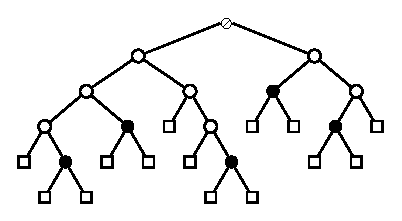
\includegraphics{bt_shape.eps}
      \end{center}

    \item Nodes are of two kinds: \textbf{internal}
      ({\tiny\raisebox{1pt}{\(\oslash\)}}, \(\circ\) and \(\bullet\))
      or \textbf{external} (\(\scriptstyle \Box\)).

    \item The \textbf{root} is the only internal node without a parent
      ({\tiny\raisebox{1pt}{\(\oslash\)}}).

    \item \textbf{Leaves} (\(\bullet\)) are internal nodes whose
      children are two external nodes (\(\scriptstyle \Box\)).

  \end{itemize}

\end{slide}

\begin{slide}
  \title{Binary trees}

  \begin{itemize}

    \item Internal nodes are usually associated with some kind of
      information, whilst external nodes are not, like
      \begin{center}
        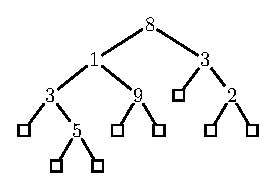
\includegraphics[bb=148 586 266 662]{bt_ex1.eps}
        \qquad
        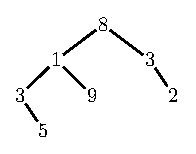
\includegraphics[bb=158 584 236 661]{bt_ex2.eps}
      \end{center}
      \centerline{\qquad\qquad\ Extended binary tree \qquad\qquad\quad Pruned binary tree}

    \item To define a binary tree in \OCaml means to write a type
      whose values are all possible binary trees. We need a
      polymorphic type, so the information stored in the tree can be
      of any type:
      \smallskip
      \begin{alltt}
        \textbf{type} \(\alpha\) tree = ...
      \end{alltt}

  \end{itemize}

\end{slide}

\begin{slide}
  \title{Binary trees in OCaml}

  \begin{itemize}

    \item We need to ponder how many shapes a binary tree can take,
      just like lists.

    \item Each shape as a value constructor and maybe some data.

    \item The empty tree is an external node, without information:
\begin{alltt}
\textbf{type} \(\alpha\) tree = Ext | ...
\end{alltt}

    \item A non\hyp{}empty tree is an internal node carrying some
      information, and which has two children:
\begin{alltt}
\textbf{type} \(\alpha\) tree = Ext | Int \textbf{of} \(\alpha\) \(\times\) \(\alpha\) tree \(\times\) \(\alpha\) tree
\end{alltt}

    \item The tree in the first figure corresponds to the
      \OCaml value
\begin{verbatim}
Int (8, Int (1, Int (3, Ext,
                            Int (5, Ext, Ext)),
                   Int (9, Ext, Ext)),
          Int (3, Ext,
                    Int (2, Ext, Ext)))
\end{verbatim}

  \end{itemize}

\end{slide}

\begin{slide}
  \title{Tree traversals}

  \begin{itemize}

    \item We may want to write an \OCaml function that sums the
      integers in a binary tree like so:
\begin{alltt}
\textbf{let rec} add t =
  \textbf{match} t \textbf{with}
    Int (n, left, right) \(\rightarrow\) n + add left + add right
  | Ext \(\rightarrow\) 0
\end{alltt}

    \item The only issue is that we wanted a function that does
      \emph{not} apply to empty trees (it is partial), but we need the
      value~\(0\) for the recursion to work.

  \end{itemize}

\end{slide}

\begin{slide}
  \title{The option type}

  \begin{itemize}

    \item We need another function that checks whether the
      \textbf{whole tree} is empty, and, if, returns a special value
      that means ``No sum is possible''.

    \item The solution is to use a predefined type called the
      \textbf{option type}:
      \smallskip
\begin{alltt}
\textbf{type} \(\alpha\) option = None | Some \textbf{of} \(\alpha\)
\end{alltt}

    \item For example, \texttt{(Some 3)} means ``There was a value,
      and it is~\texttt{3}'', whereas \texttt{None} means ``There was
      no value.''

  \end{itemize}

\end{slide}

\begin{slide}
  \title{Tree traversals}

  \begin{itemize}

    \item We can now finish our definition:
    \smallskip
\begin{alltt}
\textbf{let rec} add t =
  \textbf{match} t \textbf{with}
    Int (n,left,right) \(\rightarrow\) n + add left + add right
  | Ext \(\rightarrow\) 0

\textbf{let} add t =
  \textbf{match} t \textbf{with}
    Int (n,left,right) \(\rightarrow\) Some (n + add left + add right)
  | Ext \(\rightarrow\) None
\end{alltt}

   \item Note that the definition of the second function ``add'' hides
     the first one and uses it, because it is not recursive.

  \end{itemize}

\end{slide}

\begin{slide}
  \title{A shortcut}

  \begin{itemize}

  \item The \textbf{design pattern}
\begin{alltt}
\textbf{let rec} add t =
  \textbf{match} t \textbf{with}
     ... \(\rightarrow\) ...
\end{alltt}
      where \texttt{t} is not used on the right\hyp{}sides is quite
      common.

    \item That is why \OCaml provides a shortcut with a new keyword:
      \smallskip
\begin{alltt}
\textbf{let rec} add = \textbf{function}
  Int (n,left,right) \(\rightarrow\) n + add left + add right
| Ext \(\rightarrow\) 0

\textbf{let} add = \textbf{function}
  Int (n,left,right) \(\rightarrow\) Some (n + add left + add right)
| Ext \(\rightarrow\) None
\end{alltt}

  \end{itemize}

\end{slide}

\begin{slide}
  \title{Tree traversals (resumed)}

  Let~\texttt{t} be the tree \texttt{Int(x,l,r)}.
  \begin{itemize}

    \item The \textbf{preorder traversal} of~\texttt{t} is the list
      whose first element is~\texttt{x}, followed by the elements of
      the preorder traversal of~\texttt{l}, followed by the elements
      of the preorder traversal of~\texttt{r}. The previous tree
      yields \texttt{[8;1;3;5;9;3;2]}.

    \item The \textbf{postorder traversal} of~\texttt{t} is the list
      made of the elements of the postorder traversal of~\texttt{l},
      followed by the elements of the postorder traversal
      of~\texttt{r}, followed by~\texttt{x}. The previous tree yields
      \texttt{[5;3;9;1;2;3;8]}.

    \item The \textbf{inorder traversal} of~\texttt{t} is the list
      made of the elements of the inorder traversal of~\texttt{l},
      followed by~\texttt{x}, followed by the elements of the inorder
      traversal of~\texttt{r}. The previous tree yields
      \texttt{[3;5;1;9;8;3;2]}.

  \end{itemize}

\end{slide}

\begin{slide}
  \title{Tree traversals}

  \begin{itemize}

    \item We want to build the traversals only by pushing (consing).

    \item We must add an \textbf{auxiliary parameter}, originally set
      to the empty list, on which the contents of the nodes are pushed
      in the proper order. For preorder:
\begin{alltt}
\textbf{let} pre t s = ...
\textbf{let} pre t = pre t []
\end{alltt}

    \item This kind of extra parameter is called an
      \textbf{accumulator}, because it accumulates parts of the total
      result until the main structure (\texttt{t}) is fully traversed.

    \item We should interpret this accumulator when considering the
      call \((\fun{pre} \; t \; s)\). Let us consider the tree \(t =
      \fun{Int} (x, t_1, t_2)\) in the figures
      \begin{center}
        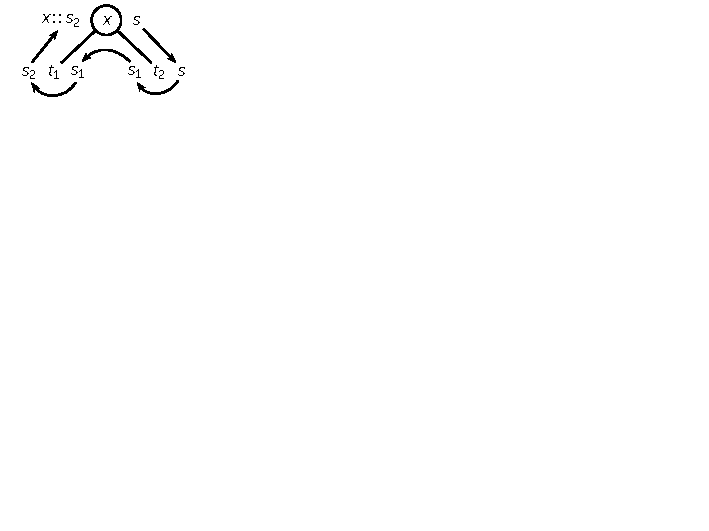
\includegraphics[trim=0 75mm 75mm -2,scale=0.9]{pre_tree.pdf}
        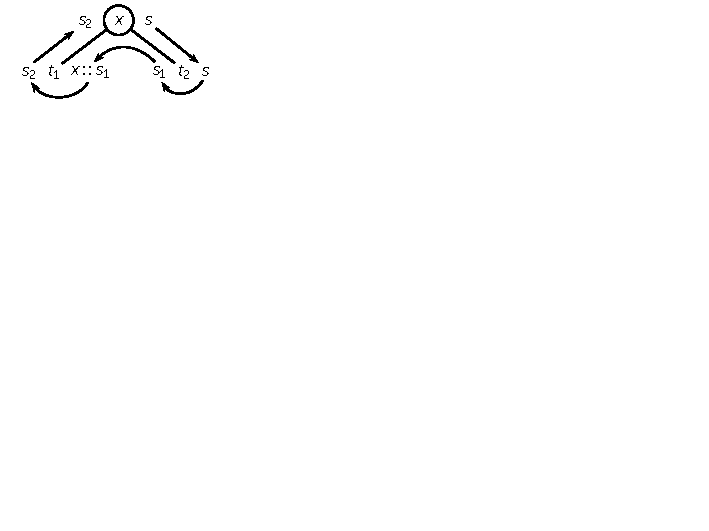
\includegraphics[trim=1cm 75mm 75mm -2,scale=0.9]{in_tree.pdf}
        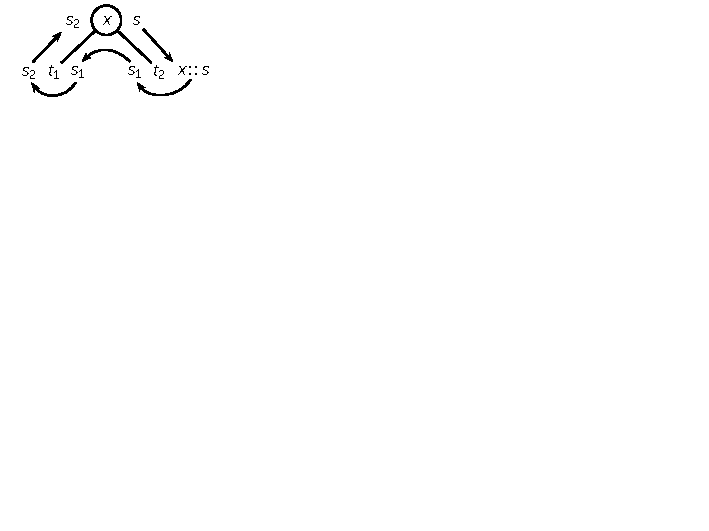
\includegraphics[trim=1cm 75mm 75mm -2,scale=0.9]{post_tree.pdf}
      \end{center}
      \centerline{Preorder (\texttt{pre}) \qquad\qquad
      Inorder (\texttt{inorder}) \qquad Postorder (\texttt{post})}

  \end{itemize}

\end{slide}

\begin{slide}
  \title{Preorder traversal}

  \begin{itemize}

    \item Each arrow is a step in the traversal and connects different
      stages of the accumulator: a downwards arrow points to the
      argument of a recursive call on the corresponding child; an
      upwards arrow points to the value of the call on the parent.

    \item For instance, the leftmost figure, the subtree~\(t_2\)
      corresponds to the recursive call \((\fun{pre} \;\; t_2 \;\;
      s)\) whose value is named~\(s_1\), which we note
      \begin{equation*}
        \fun{pre} \;\; t_2 \;\; s \;\; \twoheadrightarrow \;\; s_1
      \end{equation*}

    \item Likewise, we have \(\fun{pre} \;\; t_1 \;\; s_1 \;\;
      \twoheadrightarrow \;\; s_2\). Therefore
      \begin{equation*}
        \fun{pre} \;\; t_1 \;\; (\fun{pre} \;\; t_2 \;\; s) \;\;
        \twoheadrightarrow \;\; s_2
      \end{equation*}

    \item The root is associated with the evaluation
      \begin{equation*}
        \fun{pre} \;\;
        t \;\; s \;\; \twoheadrightarrow \;\; \cons{x}{s_2}
      \end{equation*}
      Consequently,
      \begin{equation*}
        \fun{pre} \;\; t \;\; s \;\; \equiv \;\;
        \cons{x\,}{\,\fun{pre} \;\; t_1 \;\; (\fun{pre} \;\; t_2 \;\;
          s)}.
      \end{equation*}

    \item The rules for external nodes are not shown and simply
      consist in leaving the accumulator invariant.

  \end{itemize}

\end{slide}

\begin{slide}
  \title{Preorder traversal}

  \begin{itemize}

    \item The \OCaml function for the preorder traversal of a binary
      tree is
\begin{alltt}
\textbf{let rec} pre t s =
  \textbf{match} t \textbf{with}
                Ext \(\rightarrow\) s
  | Int (x,t1,t2) \(\rightarrow\) x :: pre t1 (pre t2 s)

\textbf{let} pre t = pre t []
\end{alltt}
\smallskip

  \item If we swap the parameters \texttt{t}~and~\texttt{s} above, we
    can use the \textbf{function} construct because \texttt{t}~is not
    used on the right\hyp{}hand sides:
\begin{alltt}
\textbf{let rec} pre s = \textbf{function}
              Ext \(\rightarrow\) s
| Int (x,t1,t2) \(\rightarrow\) x :: pre (pre s t2) t1

\textbf{let} pre t = pre [] t
\end{alltt}

  \end{itemize}

\end{slide}

\begin{slide}
  \title{Inorder and postorder traversals}

  \begin{itemize}

    \item Similarly, we can derive the \OCaml function for the inorder
      traversal of a binary tree:
\begin{alltt}
\textbf{let rec} inorder s = \textbf{function}
              Ext \(\rightarrow\) s
| Int (x,t1,t2) \(\rightarrow\) inorder (x :: inorder s t2) t1

\textbf{let} inorder t = inorder [] t
\end{alltt}
\smallskip

  \item The same goes for the postorder traversal:
\begin{alltt}
\textbf{let rec} post s = \textbf{function}
              Ext \(\rightarrow\) s
| Int (x,t1,t2) \(\rightarrow\) post (post (x::s) t2) t1

\textbf{let} post t = post [] t
\end{alltt}

\end{itemize}

\end{slide}

\begin{slide}
  \label{slide:balanced}
  \title{Binary Search Trees}

  \begin{itemize}

    \item Searching in a binary tree can be costly because, in the
      worst case, the whole tree must be traversed.

    \item To improve upon the worst case, two scenarios are desirable:
      \begin{enumerate}

        \item the binary tree should be as \textbf{balanced} as
          possible, that is, the nodes should lie as close as possible
          to the root (for a given notion of distance), and

        \item at a given node, \textbf{only the left or the right
          subtree should be visited}, a decision taken solely by
          comparing the key at the root and the sought key.

      \end{enumerate}

    \item The simplest solution consists in satisfying the second
      goal, and see later how to also reach the first.

    \item A \textbf{binary search tree} is either \texttt{Empty}, or
      it is a value \texttt{BST($x$,$t_1$,$t_2$)}, such that the
      key~\(x\) is greater than or equal to the keys in the left
      subtree~\(t_1\), and lower than the keys in~\(t_2\).

  \end{itemize}

\end{slide}

\begin{slide}
  \title{Binary Search Trees}

  \begin{itemize}

    \item The definition of an \OCaml type for such trees is
      isomorphic to that of binary trees, as the ordering constraint
      cannot be expressed at the type level:
      \smallskip
\begin{alltt}
\textbf{type} \(\alpha\) bst = Empty | BST of \(\alpha\) \(\times\) \(\alpha\) bst \(\times\) \(\alpha\) bst
\textbf{type} \(\alpha\) tree = Ext | Int of \(\alpha\) \(\times\) \(\alpha\) tree \(\times\) \(\alpha\) tree
\end{alltt}

   \item Therefore, let us retain the type \texttt{tree}.

   \item The \textbf{total ordering of the keys} (that is, the fact
     that any two keys must be comparable) can be expressed at the
     \textbf{module level}, which is an advanced feature of \OCaml.

   \item We will not present modules in this lecture, although they
     are very important to write \textbf{composable software} that is
     type safe (libraries).

   \item A consequence is that the inorder traversal of a binary
     search tree is the list of its keys sorted in non\hyp{}decreasing
     order.

  \end{itemize}

\end{slide}

\begin{slide}
  \title{Binary Search Trees}

  \begin{itemize}

   \item Here is an example:
     \begin{center}
       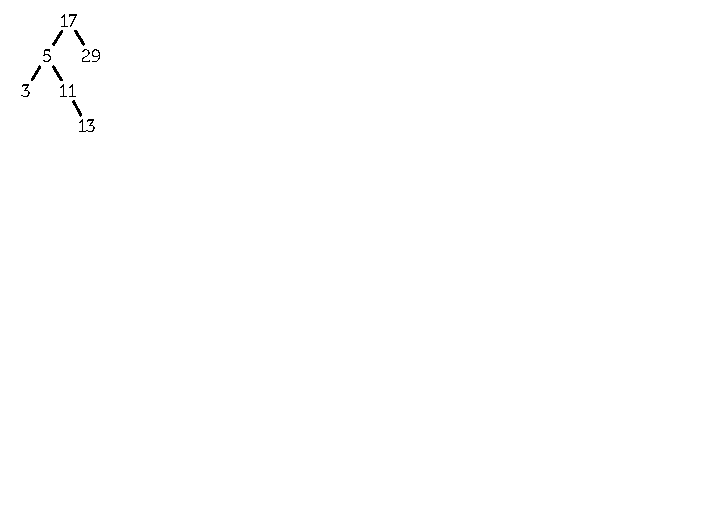
\includegraphics[trim=5mm 7cm 9cm 2mm]{bst_ex.pdf}
     \end{center}

   \item The \OCaml value for that tree is:
\begin{alltt}
\textbf{let} t =
  Int (17, Int (5, Int (3, Ext, Ext),
                      Int (11, Ext,
                                 Int (13, Ext, Ext))),
             Int (29, Ext, Ext))
\end{alltt}

   \item The inorder traversal is:

      \noindent\topin{\textbf{let} l = inorder t}

      \noindent\topout{\textbf{val} l~:~int list = [3;5;11;13;17;29]}

  \end{itemize}
\end{slide}

\begin{slide}
  \title{Searching}

  \begin{itemize}

    \item Let consider checking the \textbf{membership} of a key~\(k\)
      in a binary search tree.

    \item Any key is absent from the empty tree.

    \item If the tree is not empty, it has the shape
      \texttt{Int($x$,$t_1$,$t_2$)}.

    \item We compare~\(k\) with~\(x\): if equal, we found it; if
      lower, we resume the search on~\(t_1\), else on~\(t_2\).

    \item In \OCaml:
      \smallskip
\begin{alltt}
\textbf{let rec} mem k = \textbf{function}
  Ext \(\rightarrow\) \textbf{false}
| Int (x,t1,t2) \(\rightarrow\) \textbf{if} k < x \textbf{then} mem k t1
                       \textbf{else if} x < k \textbf{then} mem k t2
                             \textbf{else} \textbf{true}
\end{alltt}

  \end{itemize}

\end{slide}

\begin{slide}
  \title{Leaf insertion}

  \begin{itemize}

    \item Since all unsuccessful searches end at an external node, it
      is tempting to start the insertion of a unique key by an
      unsuccessful search and then grow a leaf with the new key at the
      external node we reached.

    \item If the key is already present in the tree, we decide to
      leave the tree unchanged.

    \item Let us modify the \OCaml definition for membership into
\smallskip
\begin{alltt}
\textbf{let rec} add_leaf k = \textbf{function}
  Ext \(\rightarrow\) \textcolor{red}{Int (k, Ext, Ext) (* Was "false" *)}
| Int (x,t1,t2) \(\rightarrow\)
    \textbf{if} k < x \textbf{then} \textcolor{red}{Int (x,} add_leaf k t1\textcolor{red}{, t2)}
    \textbf{else if} x < k \textbf{then} \textcolor{red}{Int (x, t1,} add_leaf k t2\textcolor{red}{)}
                    \textbf{else} \textcolor{red}{Int (x,t1,t2) (* Was "true" *)}
\end{alltt}

  \end{itemize}

\end{slide}

\begin{slide}
  \title{Leaf insertion}

  \begin{itemize}

    \item If you recall \textbf{data sharing} in the context of
      rewrite systems, you would have noticed that when the sought key
      is already in the tree, a new internal node is created
      identical, instead of sharing the existing one.

    \item Moreover, all the nodes visited before from the root also
      have been duplicated for nothing.

    \item We can remedy the first problem by using a feature of \OCaml
      patterns called \textbf{aliases}, whereby we can name a
      subpattern and use that name on the right hand\hyp{}sides of the
      rules, like so:
      \smallskip
\begin{alltt}
\textbf{let rec} add_leaf k = \textbf{function}
  Ext \(\rightarrow\) Int (k, Ext, Ext)
| Int (x,t1,t2) \textcolor{red}{\textbf{as} t} \(\rightarrow\) \textcolor{red}{(* t = Int (x,t1,t2) *)}
    \textbf{if} k < x \textbf{then} Int (x, add_leaf k t1, t2)
    \textbf{else if} x < k \textbf{then} Int (x, t1, add_leaf k t2)
                     \textbf{else} \textcolor{red}{t (* Was Int (x,t1,t2) *)}
\end{alltt}

  \end{itemize}

\end{slide}

\begin{slide}
  \title{Root insertion}

  \begin{itemize}

    \item If recently inserted keys are looked up, the cost is
      relatively high because these keys are leaves or close to a
      leaf.

    \item In this scenario, instead of inserting a key as a leaf, it
      is better to insert it as a root.

    \item The idea is to perform a leaf insertion and, on the way back
      to the root (that is to say, after the recursive calls are
      evaluated, one after the other), we perform rotations to bring
      the inserted node up to the root.

    \item More precisely, if the node was inserted in a left subtree,
      then a \textbf{right rotation} brings it one level up, otherwise
      a \textbf{left rotation} has the same effect.

    \item The composition of these rotations brings the leaf to the
      root.

  \end{itemize}

\end{slide}

\begin{slide}
  \title{Right rotation}

  \begin{itemize}

    \item The right rotation can be depicted as
      \begin{center}
        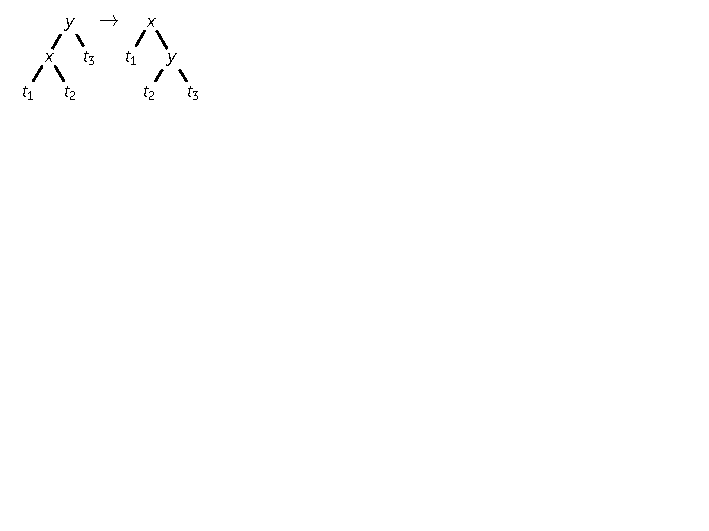
\includegraphics[trim=5mm 73mm 7cm 0]{rotr.pdf}
      \end{center}

    \item We can see that \(x\)~goes ``up'' and \(y\)~goes ``down''
      one level (this is a local transformation).

    \item It is defined in \OCaml as
      \smallskip
\begin{alltt}
\textbf{let} rotr = \textbf{function}
  Ext \(\rightarrow\) Ext
| Int (y, Int(x,t1,t2), t3) \(\rightarrow\) Int (x, t1, Int(y,t2,t3))
\end{alltt}

  \end{itemize}

\end{slide}

\begin{slide}
  \title{Left rotation}

  \begin{itemize}

    \item The left rotation can be depicted as
      \begin{center}
        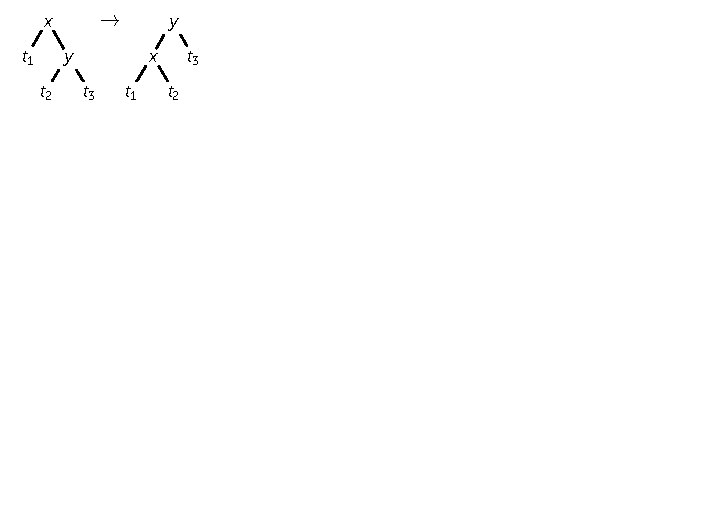
\includegraphics[trim=5mm 73mm 7cm 0]{rotl.pdf}
      \end{center}

    \item We can see that \(x\)~goes ``down'' and \(y\)~goes ``up''
      one level (this is a local transformation).

    \item It is defined in \OCaml as
      \smallskip
\begin{alltt}
\textbf{let} rotl = \textbf{function}
  Ext \(\rightarrow\) Ext
| Int (x, t1, Int(y,t2,t3)) \(\rightarrow\) Int (y, Int(x,t1,t2), t3)
\end{alltt}


  \item Left and right rotations are the \textbf{inverse} of each other:
    \begin{equation*}
      \forall t. \fun{rotl} \;\; (\fun{rotr} \;\; t) \;\; \equiv \;\;
      \fun{rotr} \;\; (\fun{rotl} \;\; t) \;\; \equiv \;\;t.
    \end{equation*}

  \end{itemize}

\end{slide}

\begin{slide}
  \title{Root insertion (resumed)}

  Let us consider an example, where \(7\)~is first added as a leaf,
  and then a series of rotations, left and right, bring it to the
  root:
  \begin{center}
    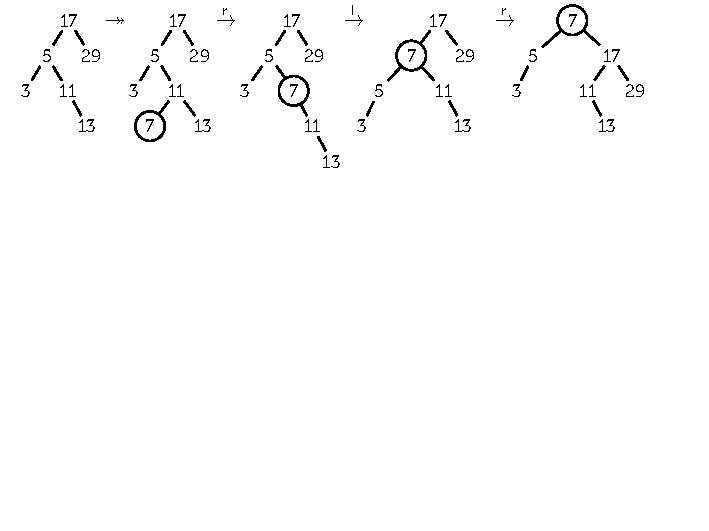
\includegraphics[trim=5mm 62mm 15mm 0]{insr_ex.pdf}
  \end{center}
  \begin{itemize}

    \item Remark that the transitive closure
      \;\((\twoheadrightarrow)\) captures the preliminary leaf
      insertion, \((\xrightarrow{\textsf{r}})\) is a right rotation
      and \((\xrightarrow{\textsf{l}})\) is a left rotation, both
      applied to the node containing~\(7\).

    \item Note also that the inorder traversal of all those trees
      remains invariant and a sorted list.

  \end{itemize}

\end{slide}

\begin{slide}
  \title{Root insertion}

  It is now a simple matter to modify the definition of
  \fun{add\_leaf} so it becomes root insertion \fun{add\_root} as follows:
\begin{alltt}
\textbf{let rec} add_root k = \textbf{function}
  Ext \(\rightarrow\) Int (k, Ext, Ext)
| Int (x,t1,t2) \textbf{as} t \(\rightarrow\)
    \textbf{if} k < x \textbf{then} \textcolor{red}{rotr (}Int (x, add_root k t1, t2)\textcolor{red}{)}
    \textbf{else if} x < k \textbf{then} \textcolor{red}{rotl (}Int (x, t1, add_root k t2)\textcolor{red}{)}
                    \textbf{else} t
\end{alltt}

We simply added a right rotation just after performing a left
insertion, and a left rotation after a right insertion.
\end{slide}

\begin{slide}
  \title{Balancing a binary search tree}

  \begin{itemize}

    \item Whether we insert a root or a leaf to a binary search tree,
      we may still obtain \textbf{degenerate trees}, that is, trees
      isomorphic to lists (each internal node has exactly one internal
      child, except the last).

    \item You may recall that we mentioned
      page~\pageref{slide:balanced} the usefulness of balancing a
      search tree, so that these extreme cases do not happen.

    \item There exist different criteria to balance a tree, the two
      most common relying on
      \begin{enumerate}

        \item the \textbf{distance} of a node to the root (the path
          length),

        \item the \textbf{weight} of a node (the number of nodes in
          its subtrees).

      \end{enumerate}

    \item Unfortunately, discussing and implementing these strategies
      would lead us too far in this lecture, but you can refer to the
      literature.

  \end{itemize}

\end{slide}

\begin{slide}
  \title{Sorting with Binary Search Trees}

  \begin{itemize}

    \item We already noticed how insertions leave the inorder
      traversal of a binary search tree unchanged.

    \item Also the inorder traversal of a binary search tree is the
      list of its keys sorted in non\hyp{}decreasing order.

    \item Combining these two facts (which can be made formal claims
      and proved), we deduce that we can use binary search trees to
      sort a list of keys chosen from a totally ordered set.

    \item We start by inserting each key in an empty binary search
      tree.

    \item Next, we collate the inorder traversal of the final tree.
      \smallskip
\begin{alltt}
\textbf{let} sort l = inorder (fold add\_leaf l Ext)
\end{alltt}

  \end{itemize}

\end{slide}

\end{document}
